\documentclass[class=article, crop=false, 12pt]{standalone}
\usepackage[subpreambles=true]{standalone}
\usepackage{../.common/common}
\allowdisplaybreaks % equation environment from amsmath can break equation between page

\author{Tony Shing}
%\pretitle{Supplementary}

\topic{Note 05 (Math for Physics)}
\title{Vector Calculus}

\version{2025} % leave blank for omitting

\begin{document}

\maketitle


\begin{overview}
    \begin{itemize}
        \item Limit of vector functions
        \item Differentiation 
        $\bcase{
            &\text{To vectors}\\
            &\text{By vectors}
        }$
        \item Curve parametrization \& Line integral
    \end{itemize}
\end{overview}




% content begins here
% Section %%%%%%%%%%%%%%%%%%%%%%%%%%%%%%%%%%%%%%%%%%%%%%%%%%%%
\section{Review: Vector Geometry}

Geometrically, vectors can be thought as objects that have both \bf{magnitude} and \bf{direction}.


\begin{minipage}[t]{0.6\linewidth}
    \hfill\\[-2em]
    \begin{itemize}
        \item We usually visualized a vector as an arrow, 
        pointing from origin to some coordinate.

    \end{itemize}
\end{minipage}
\hspace{2em}
\begin{minipage}[t]{0.15\linewidth}
    \centering
    \begin{figure}[t]
        \strut\vspace*{-\baselineskip}\newline
        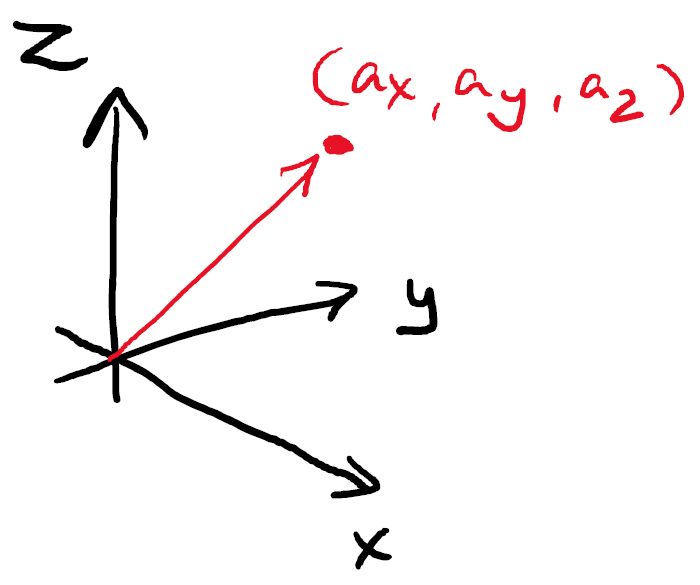
\includegraphics[width=\textwidth]{vec_arrow}
    \end{figure}
\end{minipage}


\begin{itemize}
    \item Vectors can be expressed by column matrices.
    Using row matrices is OK but mathematicians do interpret them differently.
    \aleq{
        \green{\text{prefered }\rightarrow} \ \bmat{a_x\\a_y\\a_z} \qquad\qquad
        \bmat{a_x & a_y & a_z} \ \red{\leftarrow \text{ Not prefered}}
    }    
\end{itemize}

Here are some notations and operations that you (should have) learnt about geometrical vectors.

\begin{enumerate}
    \item \bf{\ul{Norm}} (The magnitude)
    \begin{itemize}
        \item Notation: $\Vert\vvec{a}\Vert$. 
        Can also use $|\vvec{a}|$ informally.
        
        Some mathematicians are strict about that norm should use double vertical bars $\Vert\cdot\Vert$,
        while single vertical bar $|\cdot|$ is reserved for absolute value.
        But many books would just use $|\cdot|$ in both cases.

        \item Geometrically the length of the vector.
        Calculation follows Pythagoras theorem.

        \begin{center}
            \begin{minipage}{0.25\linewidth}
                \centering
                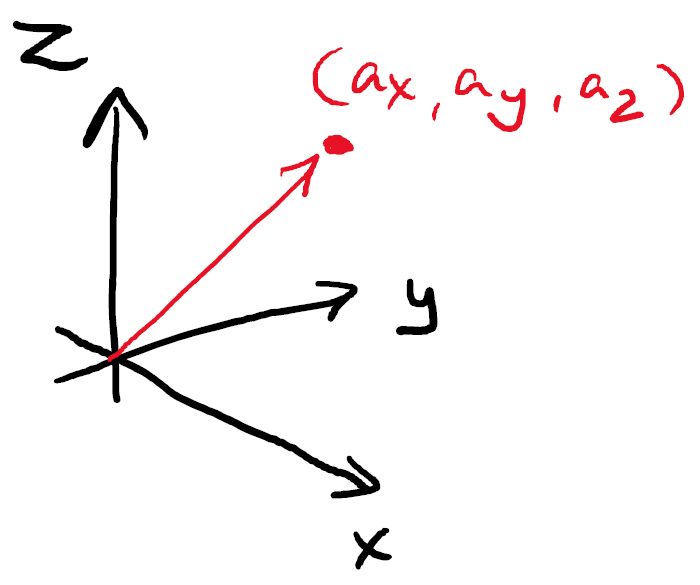
\includegraphics[width=\textwidth]{vec_arrow}
            \end{minipage}
            \begin{minipage}{0.4\linewidth}
                $\Rightarrow \qquad \red{\Vert{\vvec{a}}\Vert = \sqrt{a_x^2+a_y^2+a_z^2}}$
            \end{minipage}
        \end{center}

    \end{itemize}

    \item \bf{\ul{Unit vector}} (The direction)
    \begin{itemize}
        \item Notation: $\hhat{a}$, 
        replacing the vector arrow $\,\vvec{}\,$ with a hat $\,\hhat{}\,$.
        
        \item Formed by a vector divided by its norm (length) :  
        \blue{$\hhat{a} \equiv \frac{\vvec{a}}{\norm{\vvec{a}}}$}, 
        so that it is a vector that points in a given direction but always has norm $=1$.

    \end{itemize}


    In x-y-z coordinate, the 3 basis vectors are conventionally represented as
    \aleq{
        \hhat{x} = \bmat{1\\0\\0} \ ,\ \hhat{y} = \bmat{0\\1\\0} \ ,\ \hhat{z} = \bmat{0\\0\\1} 
    }
    
    And so any vectors in the 3D space can be expressed as a linear combination of these 3 unit vectors:
    \aleq{
        \vvec{a} = \bmat{a_x\\a_y\\a_z} 
        &= \red{a_x}\blue{\bmat{1\\0\\0}} + \red{a_y}\blue{\bmat{0\\1\\0}} + \red{a_z}\blue{\bmat{0\\0\\1}} \\
        &= \red{a_x}\blue{\hhat{x}} + \red{a_y}\blue{\hhat{y}} + \red{a_z}\blue{\hhat{z}}
    }

    Vector is a combination of \red{(magnitude)}$\times$\blue{(direction)}.\\


    \item \bf{\ul{Addition/Subtraction}}
    \begin{itemize}
        \item Operations are component-wise:
        \aleq{
            \vvec{a} \pm \vvec{b} &= (a_x\hhat{x}+a_y\hhat{y}+z\hhat{z}) \pm (b_x\hhat{x}+b_y\hhat{y}+b_z\hhat{z})\\
            &= (a_x\pm b_x)\hhat{x} + (a_y\pm b_y)\hhat{y} + (a_z\pm b_z)\hhat{z}
        }

        \item Geometrically, it can be depicted as parallelogram rule.
        
        \begin{center}
            \begin{minipage}{0.7\linewidth}
                \centering
                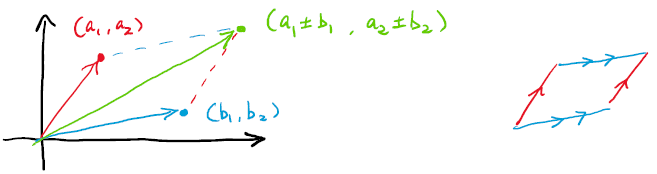
\includegraphics[width=\textwidth]{paralelogram}
            \end{minipage}
        \end{center}

    \end{itemize}
    
    \hfill\\
    \item \bf{\ul{Multiplication with constants}}
    \begin{itemize}
        \item Operations are component-wise:
        \aleq{
            k\vvec{a} &= k(a_x\hhat{x}+a_y\hhat{y}+z\hhat{z})\\
            &= (ka_x)\hhat{x} + (ka_y)\hhat{y} + (ka_z)\hhat{z}
        }

    \end{itemize}

    \begin{minipage}{0.7\linewidth}
        \begin{itemize}
            \item Geometrically, it can be depicted as extending / contracting the vector in the same/opposite direction.
        \end{itemize}
    \end{minipage}
    \hspace{2em}
    \begin{minipage}{0.2\linewidth}
        \centering
        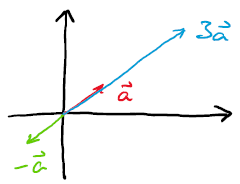
\includegraphics[width=\textwidth]{scaling}
    \end{minipage}
        
    
    
    \hfill\\
    \item \bf{\ul{Dot product}} (Scalar product)
    
    A multiplication operation between 2 vectors, that yields \ul{a number}.
    \begin{itemize}
        \item With the components of both vectors, it can be calculated as 
        \aleq{
            \vvec{a}\cdot \vvec{b} &= a_xb_x + a_yb_y + a_zb_z\\
            &= \bmat{a_x & a_y & a_z}\bmat{b_x\\b_y\\b_z}
        }
        Note that dot product is symmetric, i.e. $\vvec{a}\cdot\vvec{b} = \vvec{b}\cdot\vvec{a}$.

        \item Geometrically, dot product can be viewed as projection of one vector onto the other
        \begin{center}
            \begin{minipage}{0.4\linewidth}
                \aleq{
                    \vvec{a}\cdot\vvec{b} = \norm{\vvec{a}}\norm{\vvec{b}}\cos{\theta}
                }
            \end{minipage}
            \begin{minipage}{0.1\linewidth}
                \centering
                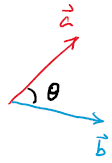
\includegraphics[width=\textwidth]{dot}
            \end{minipage}
        \end{center}

        where $\theta$ is the angle between the vectors.
        Specifically if one of them is a unit vector,
        computing dot product yields the component of another vector in this unit vector's direction.
        \begin{center}
            \begin{minipage}{0.4\linewidth}
                \aleq{
                    \vvec{a}\cdot \hhat{b} = \norm{\vvec{a}}\cus[blue]{\norm{\hhat{b}}}{=1}\cos{\theta} 
                    = \norm{\vvec{a}}\cos{\theta}
                }
            \end{minipage}
            \hspace{2em}
            \begin{minipage}{0.15\linewidth}
                \centering
                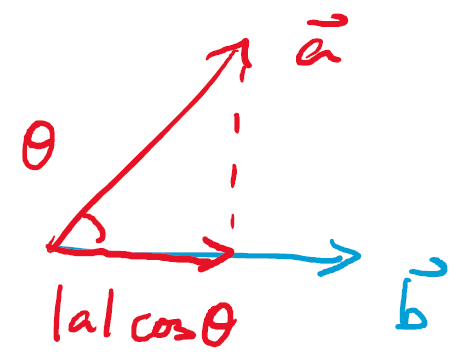
\includegraphics[width=\textwidth]{dot_proj}
            \end{minipage}
        \end{center}
        

        We can use this property to separate components of a vector. E.g.
        \aleq{
            \vvec{a}\cdot \hhat{x} = \bmat{a_x & a_y & a_z}\cdot \hhat{x} 
            = \bmat{a_x & a_y & a_z}\bmat{1\\0\\0} = a_x = \text{ x component of }\vvec{a}
        }

        and write something like
        \aleq{
            \vvec{a} = (\vvec{a}\cdot\hhat{x})\hhat{x} + (\vvec{a}\cdot\hhat{y})\hhat{y} + (\vvec{a}\cdot\hhat{z})\hhat{z}
        }
    \end{itemize}


    \hfill\\
    \item \bf{\ul{Cross product}} (Vector product)
    
    A multiplication operation between 2 vectors, that yields \ul{a new vector}. 

    \begin{itemize}
        \item Cross product is \ul{only defined in 3D space.} 
    
        {\scriptsize (There are definitions extended for vectors in higher dimension but they are totally out of our scope)}
    
        \item With the components of both vectors, 
        it can be calculated by determinant:
        \aleq{
            \vvec{c} = \vvec{a}\cross\vvec{b} = 
            \bdet{\hhat{x} & \hhat{y} & \hhat{z} \\ a_x & a_y & a_z \\ b_x & b_y & b_z}
        }
        Note that cross product is antisymmetric, i.e. $\vvec{a}\cross\vvec{b} = -\vvec{b}\cross\vvec{a}$.

        \item Geometrically, cross product outputs a vector that is perpendicular to the plane spanned by the original 2 vectors.
        This vector has a magnitude $\norm{\vvec{c}}=\norm{\vvec{a}}\norm{\vvec{b}}\sin{\theta}$.

        \begin{center}
            \begin{minipage}{0.55\linewidth}
                \centering
                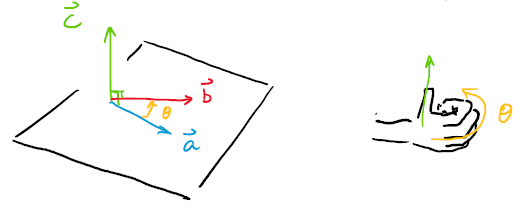
\includegraphics[width=\textwidth]{cross}
            \end{minipage}
        \end{center}

        The direction of the product vector can be found using right hand grip rule. 
        The curl of the 4 fingers represent the rotation direction from $\vvec{a}$ to $\vvec{b}$.
        Then the thumb will point into the direction of $\vvec{c}$.\\

        \begin{example} (Order of $\hhat{x}$-$\hhat{y}$-$\hhat{z}$)\\

            Conventionally, the direction of the 3 unit vectors follow the order of right hand grip rule.
            We can verify with cross product:
            \aleq{
                \hhat{x}\cross\hhat{y} = \bdet{\hhat{x} & \hhat{y} & \hhat{z} \\ 1 & 0 & 0 \\ 0 & 1 & 0} = \hhat{z}
            }
            The same for $\hhat{y}\cross\hhat{z}=\hhat{x}$ and $\hhat{z}\cross\hhat{x}=\hhat{y}$.

        \end{example}

    \end{itemize}

\end{enumerate}


\linesep
\newpage
% Section %%%%%%%%%%%%%%%%%%%%%%%%%%%%%%%%%%%%%%%%%%%%%%%%%%%%
\section{Limits on Vector Functions}

\bf{\ul{On Single Variable Vector Function}}\\

The definition of limit implies that when the input $t$ is getting closer to $t_0$,
then the output of the function $\vvec{F}(t)$, as a vector, 
is getting closer to match on a "limiting" vector $\vvec{L}$.

\aleq{
    \lim_{t\to t_0} \vvec{F}(t) = \vvec{L} \Leftrightarrow 
    \substack{}\text{ When }t\text{ approaches }t_0
}

\begin{center}
    \begin{minipage}{0.5\linewidth}
        \centering
        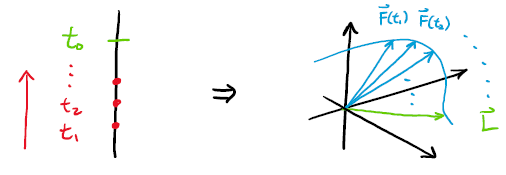
\includegraphics[width=\textwidth]{limit}
    \end{minipage}
\end{center}

Equivalently, 
it implies that the distance between $\vvec{F}(t)$ and $\vvec{L}$ need to be as small as possible
\aleq{
    &\lim_{t\to t_0} \norm{\vvec{F}(t)-\vvec{L}} = 0\\
    \Leftrightarrow\  &\lim_{t\to t_0}\sqrt{(F_x(t)-L_x)^2 + (F_y(t)-L_y)^2 + (F_z(t)-L_z)^2}\\
    \Leftrightarrow\  &\bcase{
        \lim_{t\to t_0} \norm{F_x(t)-L_x} &= 0\\
        \lim_{t\to t_0} \norm{F_y(t)-L_y} &= 0\\
        \lim_{t\to t_0} \norm{F_z(t)-L_z} &= 0
    }
}
It is the same requiring all 3 components to independently approach their own limits.

\hfill\\
\bf{\ul{On Multivariable Vector Function}}\\

The definition and notation is similar (but picture is hard to visualize).
\aleq{
    \lim_{\tkn{inputx}{(\cul[red]{x_1,x_2,...,x_n})}\to\tkn{inputa}{(\cul[red]{a_1,a_2,...,a_n})}} 
    \tkn{outputF}{\cul[blue]{\vvec{F}(x_1,x_2,...,x_n)}} = \tkn{outputL}{\cul[blue]{\vvec{L}}}
}
\addBelowArrow[red]{inputx}{inputa}{When every input $x_i$\\approach their\\target value $a_i$}
{-2ex}
\addBelowArrow[blue]{outputF}{outputL}{Each components $F_i$\\will approach their\\limit value $L_i$}
{-2ex}

\hfill\\[2em]
\linesep
% Section %%%%%%%%%%%%%%%%%%%%%%%%%%%%%%%%%%%%%%%%%%%%%%%%%%%%
\section{Vector Differentiation}

\begin{notation}
    In the following section, I will stick to the colour scheme:
    \begin{itemize}
        \item \red{red} = indices for inputs, e.g. $\red{\vvec{x}} = (x_\red{1}, x_\red{2}, ...,x_\red{n})$
        \item \blue{blue} = indices for outputs, e.g. $\blue{\vvec{F}} = (F_\blue{1}, F_\blue{2}, ...,F_\blue{n})$
    \end{itemize}
\end{notation}

     
%%%%%%%%%%%%%%
\subsection{Differentiation on Vector Functions}

%%%%%%%%%%%%%%
\subsubsection{On Single Variable Vector Function}

Here we let the functions to have $n$ components $F_\blue{1}(t)$ to $F_\blue{n}(t)$,
using unit vectors $\hhat{u}_\blue{1}$ to $\hhat{u}_\blue{n}$.
\aleq{
    \blue{\vvec{F}}(t) = F_\blue{1}(t)\hhat{u}_\blue{1} + F_\blue{2}(t)\hhat{u}_\blue{2} + ... + F_\blue{n}(t)\hhat{u}_\blue{n}
}

The differention, by limit definition, is 
\aleq{
    \dvv{\blue{\vvec{F}}}{t} &= \lim_{\Delta t\to 0} \qty[\frac{\blue{\vvec{F}}(t+\Delta t) - \blue{\vvec{F}}(t)}{\Delta t}]\\
    &= \lim_{\Delta t\to 0}\qty[\frac{F_\blue{1}(t+\Delta t) - F_\blue{1}(t)}{\Delta t}]\hhat{u}_\blue{1}
        + \lim_{\Delta t\to 0}\qty[\frac{F_\blue{2}(t+\Delta t) - F_\blue{2}(t)}{\Delta t}]\hhat{u}_\blue{2}
        + \dots\\
        %
    &= \qty[\dvv{t}F_\blue{1}(t)]\hhat{u}_\blue{1} 
        + \qty[\dvv{t}F_\blue{2}(t)]\hhat{u}_\blue{2} +\dots
        + \qty[\dvv{t}F_\blue{n}(t)]\hhat{u}_\blue{n}\\[1em]
        %
    &= \bmat{\dvv{F_\blue{1}}{t} \\[1em] \dvv{F_\blue{2}}{t} \\ \vdots \\ \dvv{F_\blue{n}}{t}}
        %
    = \dvv{t}\bmat{F_\blue{1}(t)\\F_\blue{2}(t)\\\vdots\\F_\blue{n}(t)}
    %
    = \text{ Differentiate each component individually}
}

The rules for calculation are basically the same as in single variable functions.

\begin{itemize}
    \item \ul{Addition/Subtraction} : 
    $\dvv{t}\qty[\vvec{F}(t)\pm\vvec{G}(t)] = \dvv{t}\vvec{F}(t) \pm \dvv{t}\vvec{G}(t)$

    \item \ul{Scaling} :
    $\dvv{t}\qty[k\vvec{F}(t)] = k\dvv{t}\vvec{F}(t)$

    \item \ul{Product rule} : One product rule for each kind of muliplication between vectors.
    \aleq{
        \dvv{t}\qty[\vvec{F}(t)\cdot \vvec{G}(t)] &= 
        \qty[\dvv{t}\vvec{F}(t)]\cdot\vvec{G}(t) + \vvec{F}(t)\cdot \qty[\dvv{t}\vvec{G}(t)]\\
        %
        \dvv{t}\qty[\vvec{F}(t)\cross \vvec{G}(t)] &= 
        \cus[red]{\qty[\dvv{t}\vvec{F}(t)]\cross\vvec{G}(t) + \vvec{F}(t)\cross \qty[\dvv{t}\vvec{G}(t)]}
        {\mstack{\text{"}F\cross G\text{" must stay the same order}\\\text{because order matters in cross Product}}}
    }
    (And there is no quotient rule, obviously.)

\end{itemize}

%%%%%%%%%%%%%%
\subsubsection{On Multivariable Vector Function}

The major difference is that there is one partial differentiation per input.
\aleq{
    \bcase{
        \cbox[gray]{\pdvv{x_\red{1}}\blue{\vvec{F}}(x_\red{1},...,x_m)}
        &= \pdvv{x_\red{1}}F_\blue{1}(x_\red{1},...,x_m)\hhat{u}_\blue{1}
            + \pdvv{x_\red{1}}F_\blue{2}(x_\red{1},...,x_m)\hhat{u}_\blue{2}
            + \dots
            + \pdvv{x_\red{1}}F_\blue{n}(x_\red{1},...,x_m)\hhat{u}_\blue{n}
        \\
        \vdots\quad\qquad &= \qquad\qquad\vdots \\
        %
        \cbox[gray]{\pdvv{x_\red{m}}\blue{\vvec{F}}(x_1,...,x_\red{m})}
        &= \pdvv{x_\red{m}}F_\blue{1}(x_1,...,x_\red{m})\hhat{u}_\blue{1}
            + \pdvv{x_\red{m}}F_\blue{2}(x_1,...,x_\red{m})\hhat{u}_\blue{2}
            + \dots
            + \pdvv{x_\red{m}}F_\blue{n}(x_1,...,x_\red{m})\hhat{u}_\blue{n}
    }
}

To make their expression easier to read,
we can write them as column matrices.
\aleq{
    \pdvv{\blue{\vvec{F}}}{x_\red{1}}
    = \bmat{\pdvv{F_\blue{1}}{x_\red{1}} \\[1em] \pdvv{F_\blue{2}}{x_\red{1}} \\ \vdots \\ \pdvv{F_\blue{n}}{x_\red{1}}}
    \quad,\quad
    \pdvv{\blue{\vvec{F}}}{x_\red{2}}
    = \bmat{\pdvv{F_\blue{1}}{x_\red{2}} \\[1em] \pdvv{F_\blue{2}}{x_\red{2}} \\ \vdots \\ \pdvv{F_\blue{n}}{x_\red{2}}}
    \quad,\quad\dots\quad,\quad
    \pdvv{\blue{\vvec{F}}}{x_\red{m}}
    = \bmat{\pdvv{F_\blue{1}}{x_\red{m}} \\[1em] \pdvv{F_\blue{2}}{x_\red{m}} \\ \vdots \\ \pdvv{F_\blue{n}}{x_\red{m}}}
}

And join each column into one big matrix:
\aleq{
    \pdvv{\blue{\vvec{F}}}{\red{\vvec{x}}}
    =
    \tkbmat{
        \pdvv{F_\blue{1}}{x_\red{1}} \& \pdvv{F_\blue{1}}{x_\red{2}} \& \cdots \& \pdvv{F_\blue{1}}{x_\red{m}} \\
        \pdvv{F_\blue{2}}{x_\red{1}} \& \pdvv{F_\blue{2}}{x_\red{2}} \& \cdots \& \pdvv{F_\blue{2}}{x_\red{m}} \\
        \vdots \& \vdots \& \ddots \& \vdots \\
        \pdvv{F_\blue{n}}{x_\red{1}} \& \pdvv{F_\blue{n}}{x_\red{2}} \& \cdots \& \pdvv{F_\blue{n}}{x_\red{m}} \\
    }{
        \draw[<->, draw=red] (m-4-1.south west |- m.south) to node[pos=0.5, below, align=center, red]{$m$ columns for\\function with $m$ inputs} (m-4-4.south east |- m.south);
        \coordinate (e) at ($(m.east) + (3ex,0)$) ;
        \draw[<->, draw=blue] (m-1-4.north east -| e) to node[pos=0.5, right, align=center, blue]{$n$ rows for\\function with\\$n$ components} (m-4-4.south east -| e);
    }
}
\begin{center}
    (This matrix is called \bf{Jacobian matrix})
\end{center}




\hfill\\
%%%%%%%%%%%%%%
\subsection{Differentiaton by Vector - Gradient}

%%%%%%%%%%%%%%
\subsubsection{On Multivariable Scalar Function}

Recall the definition of partial differentiation
\aleq{
    \pdv{x}f(x,y) = \lim_{\Delta x\to 0} \frac{f(x+\Delta x,y)-f(x,y)}{\Delta x}
    = \text{ Slope in x direction}\\
    \pdv{y}f(x,y) = \lim_{\Delta y\to 0} \frac{f(x,y+\Delta y)-f(x,y)}{\Delta y}
    = \text{ Slope in y direction}
}

What if we want the slope in an arbituary direction?

\begin{center}
    \begin{minipage}{0.7\linewidth}
        \centering
        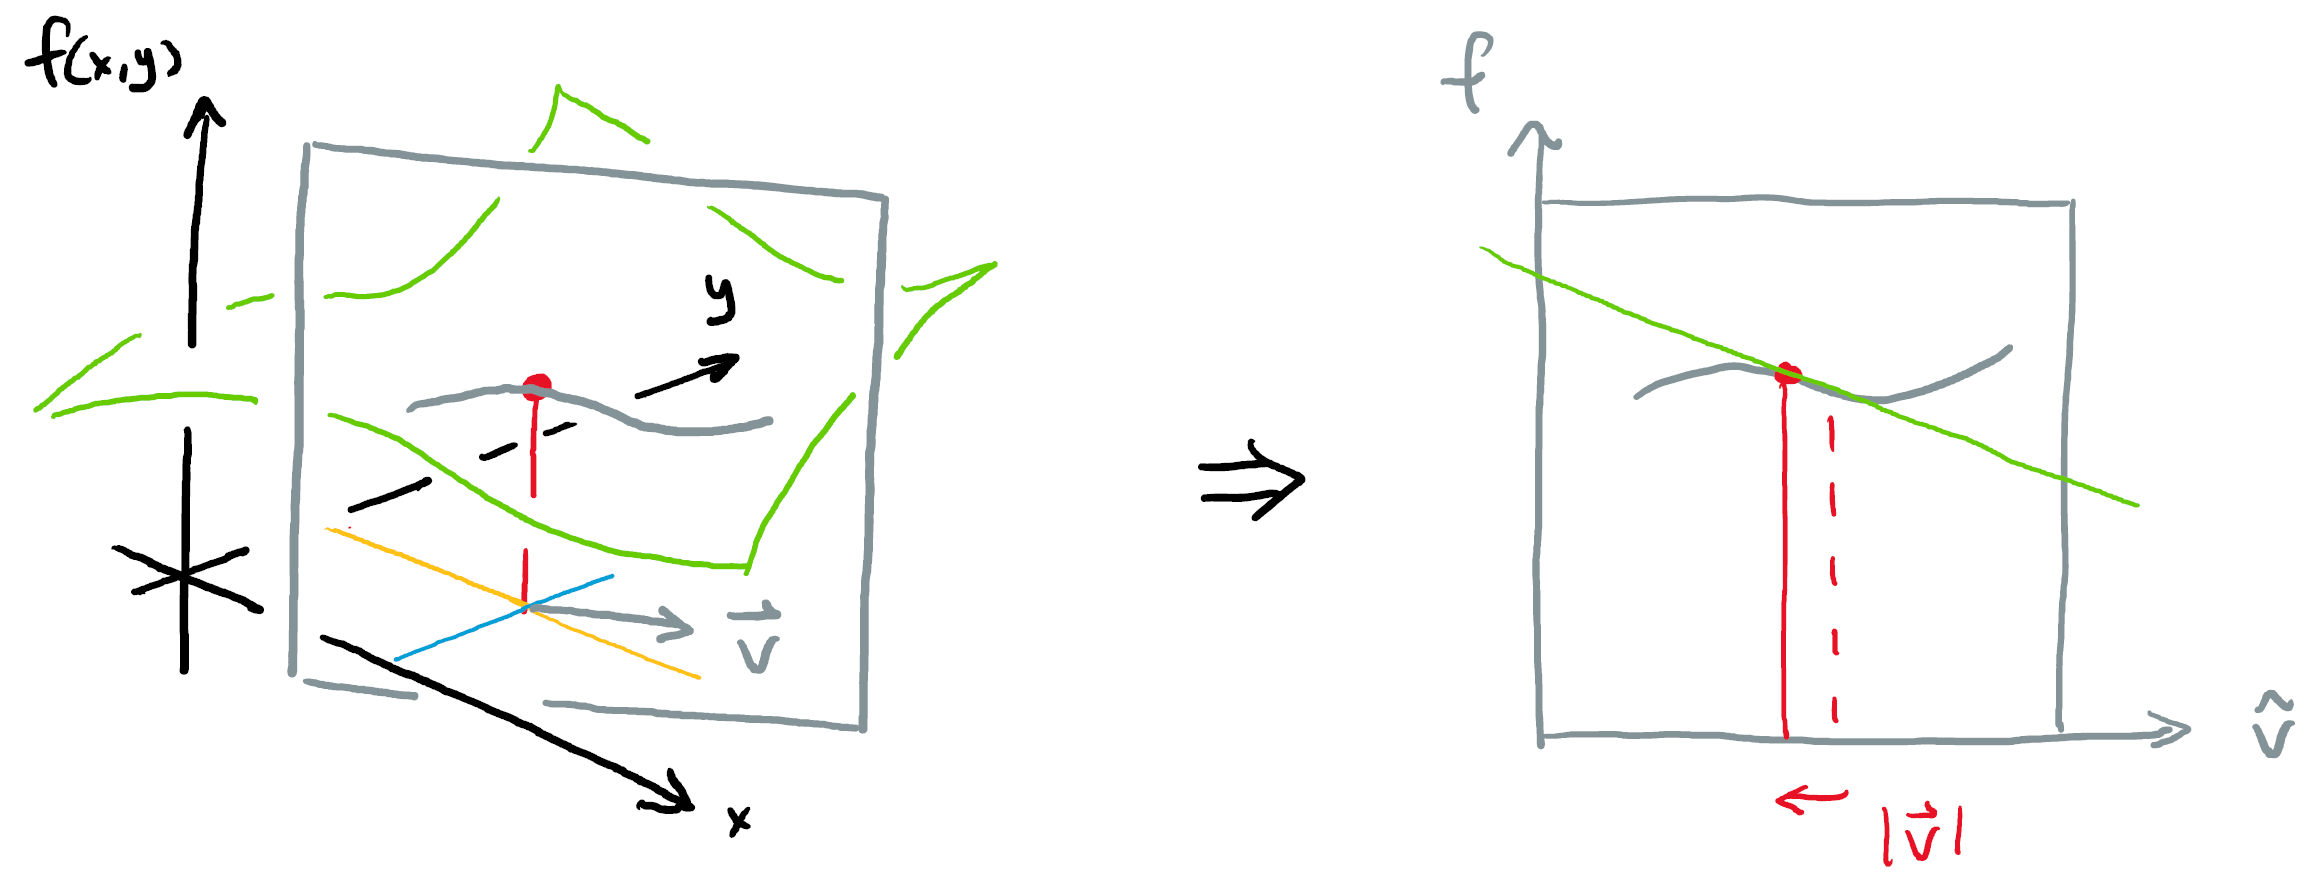
\includegraphics[width=\textwidth]{grad_plane}
    \end{minipage}
\end{center}

Suppose we want to find the slope along the direction of some vector $\vvec{v}$.
We know $\vvec{v}$ can be decomposed into component form of $\hhat{x}$/$\hhat{y}$.


\begin{center}
    \begin{minipage}{0.5\linewidth}
        \aleq{
            \vvec{v} &= v_x\hhat{x} + v_y\hhat{y}\\
            &= (\norm{\vvec{v}}\cos{\theta})\hhat{x} + (\norm{\vvec{v}}\sin{\theta})\hhat{y}
        }
    \end{minipage}
    \begin{minipage}{0.2\linewidth}
        \centering
        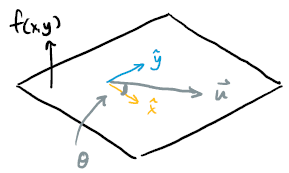
\includegraphics[width=\textwidth]{grad_u}
    \end{minipage}
\end{center}

\hfill\\
And the unit vector of $\hhat{v}$ can be expressed as 
\aleq{
    \hhat{v} = \frac{\vvec{v}}{\norm{\vvec{v}}} 
    = (\cos{\theta})\hhat{x} + (\sin{\theta})\hhat{y} = \bmat{\cos{\theta}\\\sin{\theta}}
}

To find the slope along $\vvec{v}$, 
first vary $f(x,y)$ to $f(x+v_x, y+v_y)$,
and then divide by $\norm{\vvec{v}}$. 
Finally limit $\norm{\vvec{v}} \to 0$ to turn it into differentiation.

\addArrow[red]{Du}{(0,-3ex)}{\scriptsize Just a notation\\[-1ex]\scriptsize of differentiating\\[-1ex]\scriptsize in $\vvec{v}$'s direction}
{(0,-1.5ex)}{(0,-1.5ex)}
\aleq{
    \tkn{Du}{\cul[red]{D_{\hhat{v}}}} f(x,y) 
    &= \lim_{\norm{\vvec{v}} \to 0} \frac{f(x+v_x, y+v_y)-f(x,y)}{\norm{\vvec{v}}}\\[1em]
    %
    &= \lim_{\norm{\vvec{v}} \to 0} \frac{f(x+v_x, y+v_y)\blue{-f(x,y+v_y)}}{\norm{\vvec{v}}}
        + \lim_{\norm{\vvec{v}} \to 0} \frac{\blue{f(x, y+v_y)}-f(x,y)}{\norm{\vvec{v}}}\\[1em]
    %
    &= \lim_{\norm{\vvec{v}} \to 0} \frac{f(x+v_x, y+v_y)-f(x,y+v_y)}{\blue{v_x}}\blue{\cos{\theta}}
        + \lim_{\norm{\vvec{v}} \to 0} \frac{f(x, y+v_y)-f(x,y)}{\blue{v_y}}\blue{\sin{\theta}}\\[1em]
    %
    &= \cut[green]{\cbox[green]{\lim_{\blue{v_x} \to 0} \frac{f(\cbox[green]{x+v_x}, y+v_y)-f(\cbox[green]{x},y+v_y)}{\cbox[green]{v_x}}}}
            {\text{This is exactly partial x}}\cos{\theta}
        + \cut[yellow]{\cbox[yellow]{\lim_{\blue{v_y} \to 0} \frac{f(x, \cbox[yellow]{y+v_y})-f(x,\cbox[yellow]{y})}{\cbox[yellow]{v_y}}}}
            {\text{This is exactly partial y}}\sin{\theta}\\[1em]
    %
    &= \cul[green]{\qty(\pdvv{x}f(x,y))}\cos{\theta} + \cul[yellow]{\qty(\pdvv{y}f(x,y))}\sin{\theta}\\[1em]
    %
    &= \qty(\hhat{x}\pdvv{x}f(x,y) + \hhat{y}\pdvv{y}f(x,y)) \cdot \qty((\cos{\theta})\hhat{x} + (\sin{\theta})\hhat{y})\\[1em]
    %
    &= \tkn{indpU}{\cub[purple]{\bmat{\pdvv{x}f(x,y) & \pdvv{y}f(x,y)}}{}}
        \tkn{justU}{\cul[gray]{\bmat{\cos{\theta}\\\sin{\theta}}}}
}
\addArrow[purple]{indpU}{(0,-4ex)}{\large Some row vector independent of $\vvec{v}$}
{(0,-4ex)}{(0,-0.5ex)}
\addArrow[gray]{justU}{(5ex,0)}{\scriptsize This is just $\hhat{v}$\\[-1ex]$\scriptstyle =(\cos\theta)\hhat{x}+(\sin\theta)\hhat{y}$}
{(5ex,0)}{(5ex,0)}

\hfill\\[1.5em]
So the slope in $\vvec{v}$ direction can be computed by 
a row vector of partial D of the function, doing dot product with $\hhat{v}$.
We give a special name to this row vector: \bf{gradient vector}.
\aleq{
    \tkn{nabla}{\grad} f 
    \ \defeq\  \bmat{\pdvv{f}{x_\red{1}} & \pdvv{f}{x_\red{2}} & \cdots & \pdvv{f}{x_\red{m}}}
    \ =\ \pdvv{f}{\red{\vvec{x}}}
    \ \defeq\  \tkn{nabla2}{\text{grad }} f 
}
\addArrow[purple]{nabla2}{(0,-5ex)}{\scriptsize Sometimes we\\[-1ex]\scriptsize just write "grad"}
{(0,-1ex)}{(0,-1ex)}
\addArrow[purple]{nabla}{(0,-5ex)}{\scriptsize This symbol $\nabla$ is usually pronounced "Del",\\[-1ex]\scriptsize although it is formally called "Nabla"}
{(0,-1ex)}{(0,-1ex)}

\hfill\\[2em]
The operation to compute the gradient vector of a function is called "\bf{gradient}"
\aleq{
    \grad (\cdot) = \hhat{x}_\red{1}\pdvv{x_\red{1}}(\cdot) + \hhat{x}_\red{2}\pdvv{x_\red{2}}(\cdot)
        + \dots + \hhat{x}_\red{n}\pdvv{x_\red{n}}(\cdot)
}


\hfill\\
Here are two important facts about gradient vector:

\begin{enumerate}
    \item \bf{\ul{Gradient vector itself is NOT the slope.}}\\[0.5em]
    It is just a "property"/"charateristic" of a function,
    which we can use to obtain the function's slope at any position in any direction.
    \ul{Remind that slope is a number, not a vector.}

    \item \bf{\ul{Direction of gradient vector is the same as the maximum slope's direction.}}\\[0.5em]
    Because $\grad f\cdot \hhat{v} = \norm{\grad f}\norm{\hhat{v}}\cos{\theta} \leq \norm{\grad f}$,
    the maximum slope at any position is $\norm{\grad f}$ and this happens only if $\cos{\theta}=1$,
    i.e. $\hhat{v}$ is parallel to $\grad f$. 
    
\end{enumerate}

\begin{center}
    \begin{tabular}{|c|c|c|}
        \hline
        Gradient & Gradient Vector & Slope \\
        \hline
        $\grad (\cdot)$ & $\grad f$ & $\grad f \cdot \hhat{v}$\\
        \hline
    \end{tabular}
\end{center}


\hfill\\
%%%%%%%%%%%%%%
\subsubsection{On Multivariable Vector Function}

We can take gradient to each of the function's component:
\aleq{
    \bcase{
        \cbox[gray]{\pdvv{\red{\vvec{x}}}F_\blue{1}(x_1,...,x_m)}
        &= \hhat{x}_\red{1}\pdvv{x_\red{1}}F_\blue{1}(x_1,...,x_m)
            + \hhat{x}_\red{2}\pdvv{x_\red{2}}F_\blue{1}(x_1,...,x_m)
            + \dots
            + \hhat{x}_\red{m}\pdvv{x_\red{m}}F_\blue{1}(x_1,...,x_m)
        \\
        \vdots\quad\qquad &= \qquad\qquad\vdots \\
        %
        \cbox[gray]{\pdvv{\red{\vvec{x}}}F_\blue{n}(x_1,...,x_m)}
        &= \hhat{x}_\red{1}\pdvv{x_\red{1}}F_\blue{n}(x_1,...,x_m)
            + \hhat{x}_\red{2}\pdvv{x_\red{2}}F_\blue{n}(x_1,...,x_m)
            + \dots
            + \hhat{x}_\red{m}\pdvv{x_\red{m}}F_\blue{n}(x_1,...,x_m)
    }
}

To make their expression easier to read,
we can write them as row matrices.
\aleq{
    \pdvv{F_\blue{1}}{\red{\vvec{x}}}
    &= \bmat{\pdvv{F_\blue{1}}{x_\red{1}} & \pdvv{F_\blue{1}}{x_\red{2}} & \cdots & \pdvv{F_\blue{1}}{x_\red{m}}}
    \\[1ex]
    \pdvv{F_\blue{2}}{\red{\vvec{x}}}
    &= \bmat{\pdvv{F_\blue{2}}{x_\red{1}} & \pdvv{F_\blue{2}}{x_\red{2}} & \cdots & \pdvv{F_\blue{2}}{x_\red{m}}}
    \\ \vdots \quad &\qquad\qquad \vdots\\
    \pdvv{F_\blue{n}}{\red{\vvec{x}}}
    &= \bmat{\pdvv{F_\blue{n}}{x_\red{1}} & \pdvv{F_\blue{n}}{x_\red{2}} & \cdots & \pdvv{F_\blue{n}}{x_\red{m}}}
}

\hfill\\
And join each row into one big matrix:
\aleq{
    \pdvv{\blue{\vvec{F}}}{\red{\vvec{x}}}
    =
    \tkbmat{
        \pdvv{F_\blue{1}}{x_\red{1}} \& \pdvv{F_\blue{1}}{x_\red{2}} \& \cdots \& \pdvv{F_\blue{1}}{x_\red{m}} \\
        \pdvv{F_\blue{2}}{x_\red{1}} \& \pdvv{F_\blue{2}}{x_\red{2}} \& \cdots \& \pdvv{F_\blue{2}}{x_\red{m}} \\
        \vdots \& \vdots \& \ddots \& \vdots \\
        \pdvv{F_\blue{n}}{x_\red{1}} \& \pdvv{F_\blue{n}}{x_\red{2}} \& \cdots \& \pdvv{F_\blue{n}}{x_\red{m}} \\
    }{
        \draw[<->, draw=red] (m-4-1.south west |- m.south) to node[pos=0.5, below, align=center, red]{$m$ columns for\\function with $m$ inputs} (m-4-4.south east |- m.south);
        \coordinate (e) at ($(m.east) + (3ex,0)$) ;
        \draw[<->, draw=blue] (m-1-4.north east -| e) to node[pos=0.5, right, align=center, blue]{$n$ rows for\\function with\\$n$ components} (m-4-4.south east -| e);
    }
}
\begin{center}
    (This is again the \bf{Jacobian matrix})
\end{center}


\begin{notation}[A Short Summary]
    \centering
    \begin{tabular}{c|cc}
        & \bf{Single Variable} & \bf{Multivariable} \\
        \hline\\[-1em]
        \bf{Scalar Function} & $\dvv{f}{t}$ 
        & $\bmat{\pdvv{f}{x_\red{1}} & \pdvv{f}{x_\red{2}} & \cdots & \pdvv{f}{x_\red{m}}} $\\[1.5em]
        %
        \bf{Vector Function} & $\bmat{\dvv{F_\blue{1}}{t} \\[1em] \dvv{F_\blue{2}}{t} \\ \vdots \\ \dvv{F_\blue{n}}{t}}$ 
        & $\bmat{ 
            \pdvv{F_\blue{1}}{x_\red{1}} & \pdvv{F_\blue{1}}{x_\red{2}} & \cdots & \pdvv{F_\blue{1}}{x_\red{m}} \\[1em]
            \pdvv{F_\blue{2}}{x_\red{1}} & \pdvv{F_\blue{2}}{x_\red{2}} & \cdots & \pdvv{F_\blue{2}}{x_\red{m}} \\
            \vdots & \vdots & \ddots & \vdots \\
            \pdvv{F_\blue{n}}{x_\red{1}} & \pdvv{F_\blue{n}}{x_\red{2}} & \cdots & \pdvv{F_\blue{n}}{x_\red{m}}
        }$
    \end{tabular}
\end{notation}



\hfill\\
%%%%%%%%%%%%%%
\subsection{Chain Rule in Matrix Form}

Wtih matrix, writing chain rule for multivariable function is much cleaner.
For example, let $\vvec{g}(\vvec{f}(\vvec{x}))$ be a function compositon of 
number of variables $(\red{n}\xrightarrow{f}\green{m}\xrightarrow{g}\blue{p})$.
\aleq{
    \vvec{x} &= (\tkn{reddots}{x_\red{1}, x_\red{2},...,x_\red{n}}) \\[1ex]
    \vvec{f}(\cdots) &= (\tkn{greendots}{f_\green{1}(\red{\cdots}), f_\green{2}(\red{\cdots}),..., f_\green{m}(\red{\cdots})}) \\[1ex]
    \vvec{g}(\cdots) &= (g_\blue{1}(\green{\cdots}), g_\blue{2}(\green{\cdots}),..., g_\blue{p}(\green{\cdots}))
}
\begin{tikzpicture}[remember picture,overlay]
    \draw [decorate, pen colour={red}, line width=1.25pt, decoration={calligraphic brace, mirror, aspect=0.36, amplitude=10}] 
    ($(pic cs:reddots)+(-6ex,-1ex)$) to ($(pic cs:reddots)+(6ex,-1ex)$);
    \draw [decorate, pen colour={green}, line width=1.25pt, decoration={calligraphic brace, mirror, aspect=0.15, amplitude=10}] 
    ($(pic cs:greendots)+(-12ex,-1ex)$) to ($(pic cs:greendots)+(12ex,-1ex)$);
\end{tikzpicture}

The chain rule can be written as a matrix multiplication.
\aleq{
    \pdvv{\vvec{g}}{\vvec{x}} \ \ &= \ \ \pdvv{\vvec{g}}{\vvec{f}} \ \cdot\  \pdvv{\vvec{f}}{\vvec{x}}\\
    \qty(\substack{\blue{p}\times \red{n} \\ \text{matrix}})
    &= \qty(\substack{\blue{p}\times \green{m} \\ \text{matrix}}) \qty(\substack{\green{m}\times \red{n} \\ \text{matrix}})
}
\aleq{
    \tkbmat{
        \& \& \vdots \& \& \\
        \& \& \vdots \& \& \\
        \cdots \& \cdots \& \pdvv{g_\blue{i}}{x_\red{j}} \& \cdots \& \cdots \\
        \& \& \vdots \& \& \\
        \& \& \vdots \& \& \\
    }{
        \draw[->,draw=blue] ($(m-1-3.north east) + (1ex,0)$) to node[midway, blue, right] 
            {i\Nth row} ($(m-1-3.north east |- m-3-3.north east) + (1ex,0)$);
        \draw[->,draw=red] ($(m-3-1.south west) + (0,-0.5ex)$) to node[midway, red, below] 
            {j\Nth column} ($(m-3-1.south west-| m-3-3.south west) + (0,-0.5ex)$);
    }
    %
    &= 
    %
    \tkbmat{
        \vdots \& \vdots \& \& \& \vdots \\
        \vdots \& \vdots \& \& \& \vdots \\
        \pdv{g_\blue{i}}{f_\green{1}} \& \pdv{g_\blue{i}}{f_\green{2}} \& \cdots \& \cdots \& \pdv{g_\blue{i}}{f_\green{m}} \\
        \phantom{\vdots} \& \& \& \&  \\
        \vdots \& \vdots \& \& \& \vdots \\
    }{
        \draw[->,draw=blue] ($(m-1-3.north) + (0,0)$) to node[midway, blue, right] 
            {i\Nth row} ($(m-1-3.north|- m-3-3.north) + (0,0)$);
        \draw[->,draw=green] ($(m-3-1.south west) + (0,-0.5ex)$) to node[midway, green, below] 
            {Take every element} ($(m-3-1.south west -| m-3-5.south east) + (0,-0.5ex)$);
    }
    %
    \tkbmat{
        \cdots \& \cdots \& \pdv{f_\green{1}}{x_\red{j}} \& \phantom{\cdots} \& \cdots \\
        \cdots \& \cdots \& \pdv{f_\green{2}}{x_\red{j}} \& \& \cdots \\
        \& \& \vdots \& \& \\
        \& \& \vdots \& \& \\
        \cdots \& \cdots \& \pdv{f_\green{m}}{x_\red{j}} \& \& \cdots \\
    }{
        \draw[->,draw=red] ($(m-3-1.west) + (0,-0.5ex)$) to node[midway, red, below] 
            {j\Nth column} ($(m-3-1.west-| m-3-3.west) + (0,-0.5ex)$);
        \draw[->,draw=green] ($(m-1-3.north east) + (0.5ex,0)$) to node[midway, green, above, rotate=-90] 
            {Take every element} ($(m-1-3.north east |- m-5-3.south east) + (0.5ex,0)$);
    }
}

\newpage
As individual terms which is
\aleq{
    \pdv{g_\blue{i}}{x_\red{j}} &= \sum_{\green{k=1}}^{\green{m}}\pdvv{g_\blue{i}}{f_\green{k}}\cdot\pdvv{f_\green{k}}{x_\red{j}}\\
    &= \pdvv{g_\blue{i}}{f_\green{1}}\cdot\pdvv{f_\green{1}}{x_\red{j}}
        + \pdvv{g_\blue{i}}{f_\green{2}}\cdot\pdvv{f_\green{2}}{x_\red{j}}
        + \dots
        + \pdvv{g_\blue{i}}{f_\green{m}}\cdot\pdvv{f_\green{m}}{x_\red{j}}
}

\begin{example}
    Recall this example we have seen in note of multivariable calculus, 
    \aleq{
        \bcase{
            f(p,q) &= \sqrt{p+q} \\ \vvec{h}(u,v) &= (u^2+v, u-v)
        }
        \qquad\Rightarrow\qquad
        f(\vvec{h}(u,v)) = \sqrt{u^2+u}
    }

    We can first express their derivatives in matrix form.
    \aleq{
        \bmat{\pdvv{f}{p} & \pdvv{f}{q}} 
        &= \bmat{\dinv{2\sqrt{p+q}} & \dinv{2\sqrt{p+q}}} \\[1ex]
        %
        \bmat{\pdvv{h_1}{u} & \pdvv{h_1}{v} \\[1em] \pdvv{h_2}{u} & \pdvv{h_2}{v}}
        &= \bmat{2u & 1 \\ 1 & -1}
    }

    \hfill\\
    The chain rule is therefore expressed as 
    \aleq{
        \bmat{\pdvv{f}{u} & \pdvv{f}{v}} 
        &= 
        \bmat{\pdvv{f}{p} & \pdvv{f}{q}}
        \bmat{\pdvv{h_1}{u} & \pdvv{h_1}{v} \\[1em] \pdvv{h_2}{u} & \pdvv{h_2}{v}}\\[1ex]
        %
        &=
        \bmat{\dinv{2\sqrt{p+q}} & \dinv{2\sqrt{p+q}}}\eval_{\substack{p=u^2+v\\q=u-v}}
        \bmat{2u & 1 \\ 1 & -1}\\[1ex]
        %
        &=
        \bmat{\dfrac{2u+1}{2\sqrt{u^2+u}} & 0 }
    }
\end{example}

\begin{exercise}
    Given the functions and their composition:
    \aleq{
        \bcase{
            f(p,q) &= \sqrt{p+q} \\ \vvec{g}(t) &= (t-1, t^2)
        }
        \qquad\Rightarrow\qquad
        f(\vvec{g}(t)) = \sqrt{t^2+t-1}
    }

    Compute the derivative $\dvv{t}f(\vvec{g}(t))$, 
    this time by chain rule in the matrix expression. 

\end{exercise}


\linesep
\newpage
% Section %%%%%%%%%%%%%%%%%%%%%%%%%%%%%%%%%%%%%%%%%%%%%%%%%%%%
\section{Line Integral}

%%%%%%%%%%%%%%
\subsection{Parametrizing Curves in Space}

Recall that a single variable vector function is essentially describing a curve in a space.

\begin{center}
    \begin{minipage}{0.7\linewidth}
        \centering
        \aleq{
            \vvec{r} = (x(t), y(t))
        }
        Any point on the curve only needs 1 input ($t$) to fully locate it.\\
        \red{(Intuitively, Curve = 1D object = only 1 free variable.)}

    \end{minipage}
    \begin{minipage}{0.2\linewidth}
        \centering
        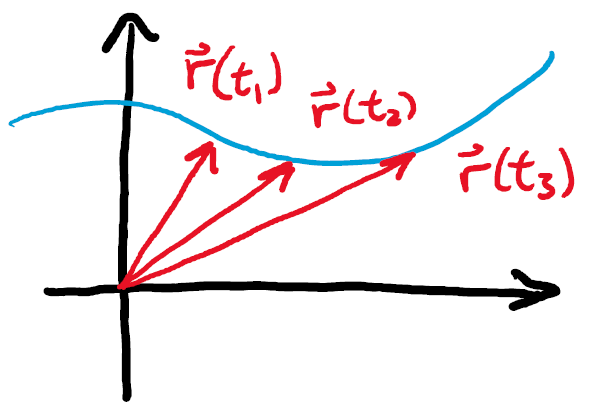
\includegraphics[width=\textwidth]{curve}
    \end{minipage}
\end{center}



Here we introduce the idea of \bf{parametrization}: 
Choose a lower-dimension coordinate system on the object to describe every point on it,
rather than using the environmental x/y/z coordinate.

\begin{center}
    \begin{minipage}{0.6\linewidth}
        \centering
        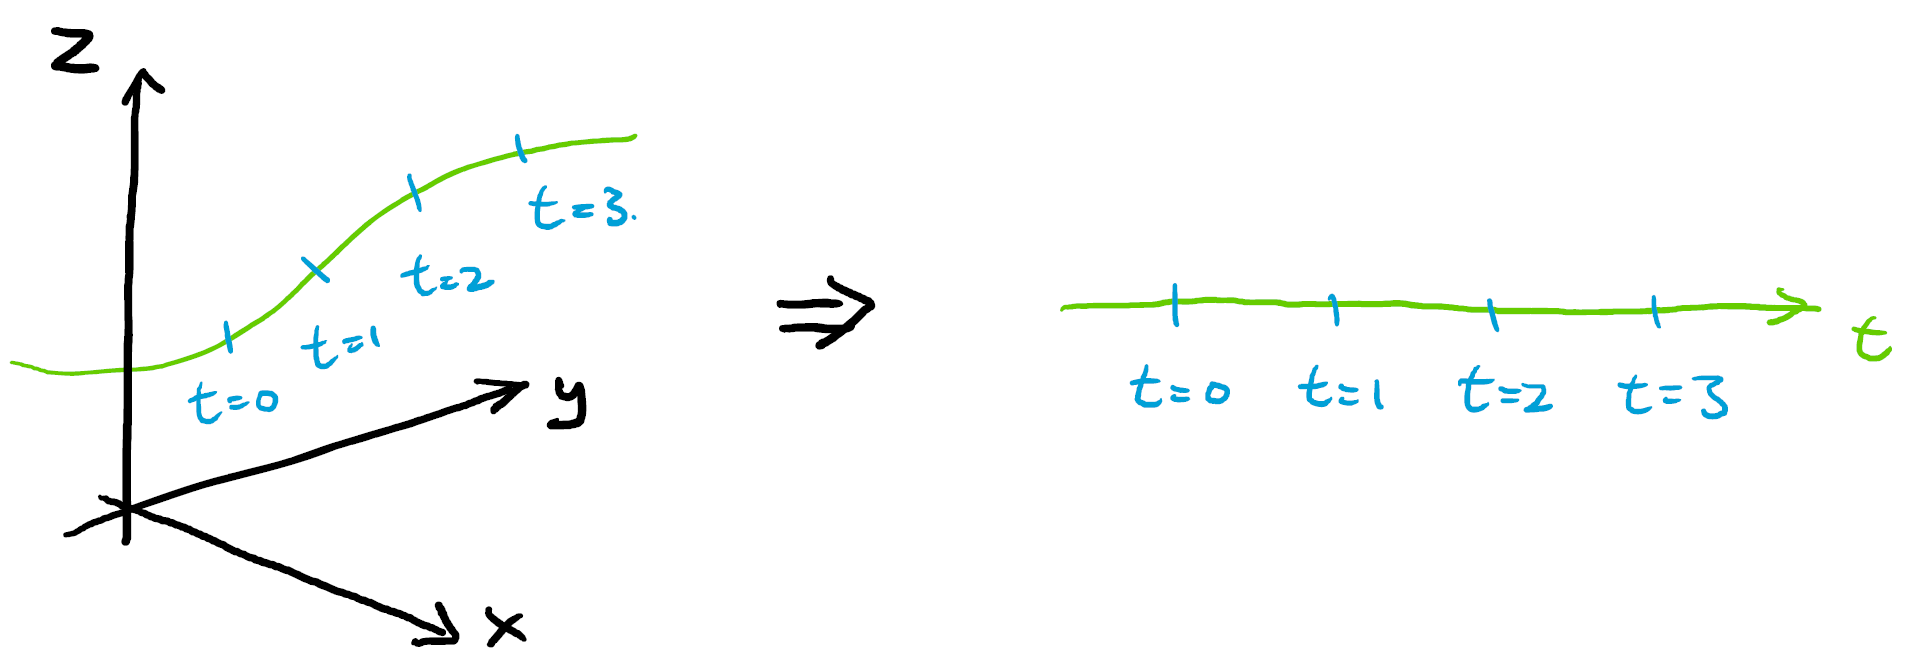
\includegraphics[width=\textwidth]{curve_para}
    \end{minipage}
\end{center}

We can also do it to higher dimension objects,
but the maths are way more complicated.

\begin{center}
    \begin{minipage}{0.6\linewidth}
        \centering
        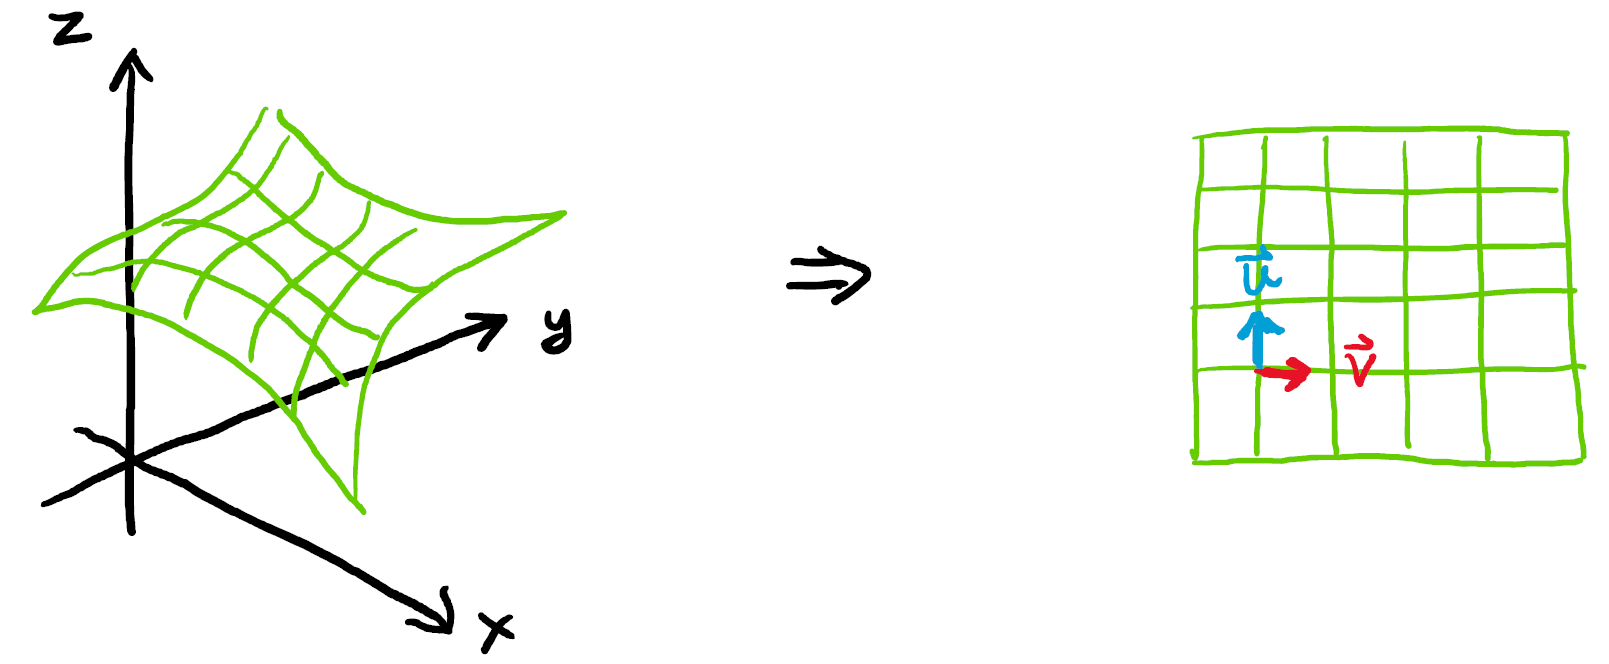
\includegraphics[width=\textwidth]{surf_para}
    \end{minipage}
\end{center}

\hfill\\[1em]
\bf{\ul{Note}}: Parametrization to an object is never unique,
because there can be infinitely many ways to choose a coordinate system.

\begin{example}
    Parametrizing the curve $y=3x^{\frac{3}{2}}$.

    \begin{itemize}
        \item Choice 1: Let $x=t^2$, then $y=3(t^2)^{\frac{3}{2}}=3t^3$ 
        $\quad\Rightarrow\quad$ Parametrize as $\vvec{r}(t)=(t^2,3t^3)$.

        \item Choice 2: Let $x=t$, then $y=3t^{\frac{3}{2}}$ 
        $\quad\Rightarrow\quad$ Parametrize as $\vvec{r}(t)=(t,3t^{\frac{3}{2}})$

        \item ...
    \end{itemize}

    There are infinitely choice of $x(t)$. 
    So the number of possible parametrization is infinite.

\end{example}

\newpage
Here are some example parametrization to common objects.
\begin{itemize}
    \item \ul{Straight line}
    \aleq{
        \vvec{r}(t) = (x(t), y(t)) = (x_0 + td_x, y_0 + td_y)
    }
    \begin{center}
        \begin{minipage}{0.28\linewidth}
            \centering
            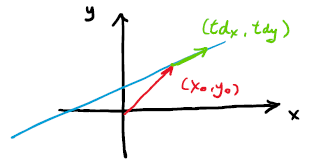
\includegraphics[width=\textwidth]{para_line}
        \end{minipage}
    \end{center}

    \item \ul{Ellipse / Circle}
    \aleq{
        \vvec{r}(t) = (x(t), y(t)) = (x_0+a\cos{(\omega t+\phi)}, y_0+b\sin{(\omega t+\phi)})
    }
    \begin{center}
        \begin{minipage}{0.4\linewidth}
            \centering
            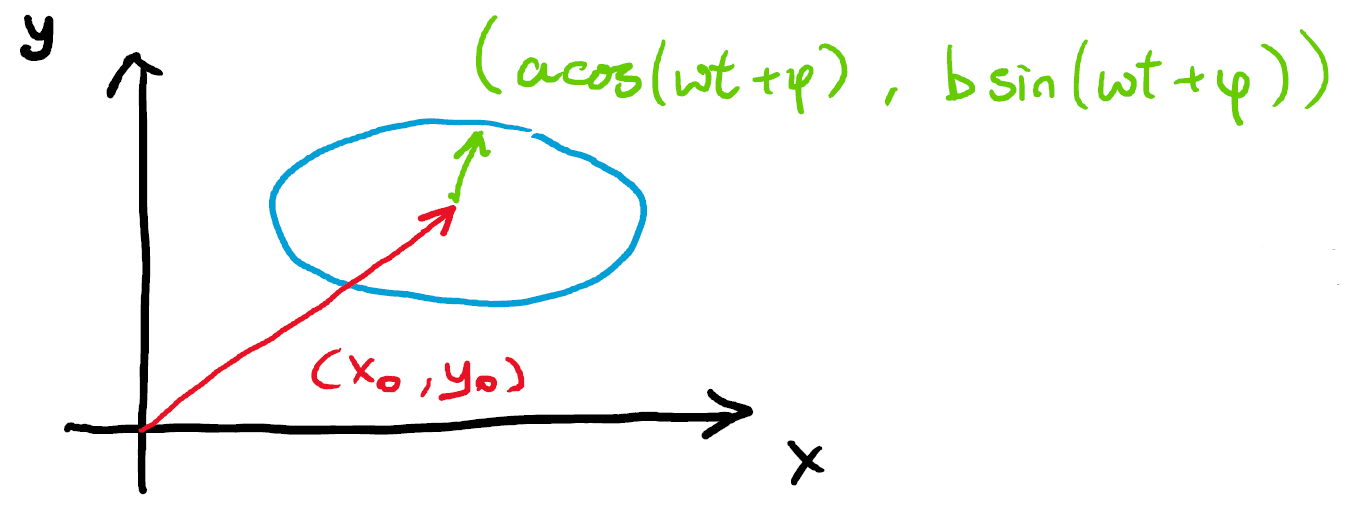
\includegraphics[width=\textwidth]{para_ellipse}
        \end{minipage}
        \begin{minipage}{0.4\linewidth}
            (If $a=b$, it becomes a circle.)
        \end{minipage}
    \end{center}

\end{itemize}

%%%%%%%%%%%%%%
\subsection{Line Integral on Scalar Functions}
Recall what we learnt in doing multiple integral

\begin{center}
    \begin{minipage}{0.45\textwidth}
        \centering
        $\displaystyle\int f(x,y)\dd{x} 
        \ =\  \mstack{\text{Integrate along x-axis}\\\text{at constant y}}$\\
        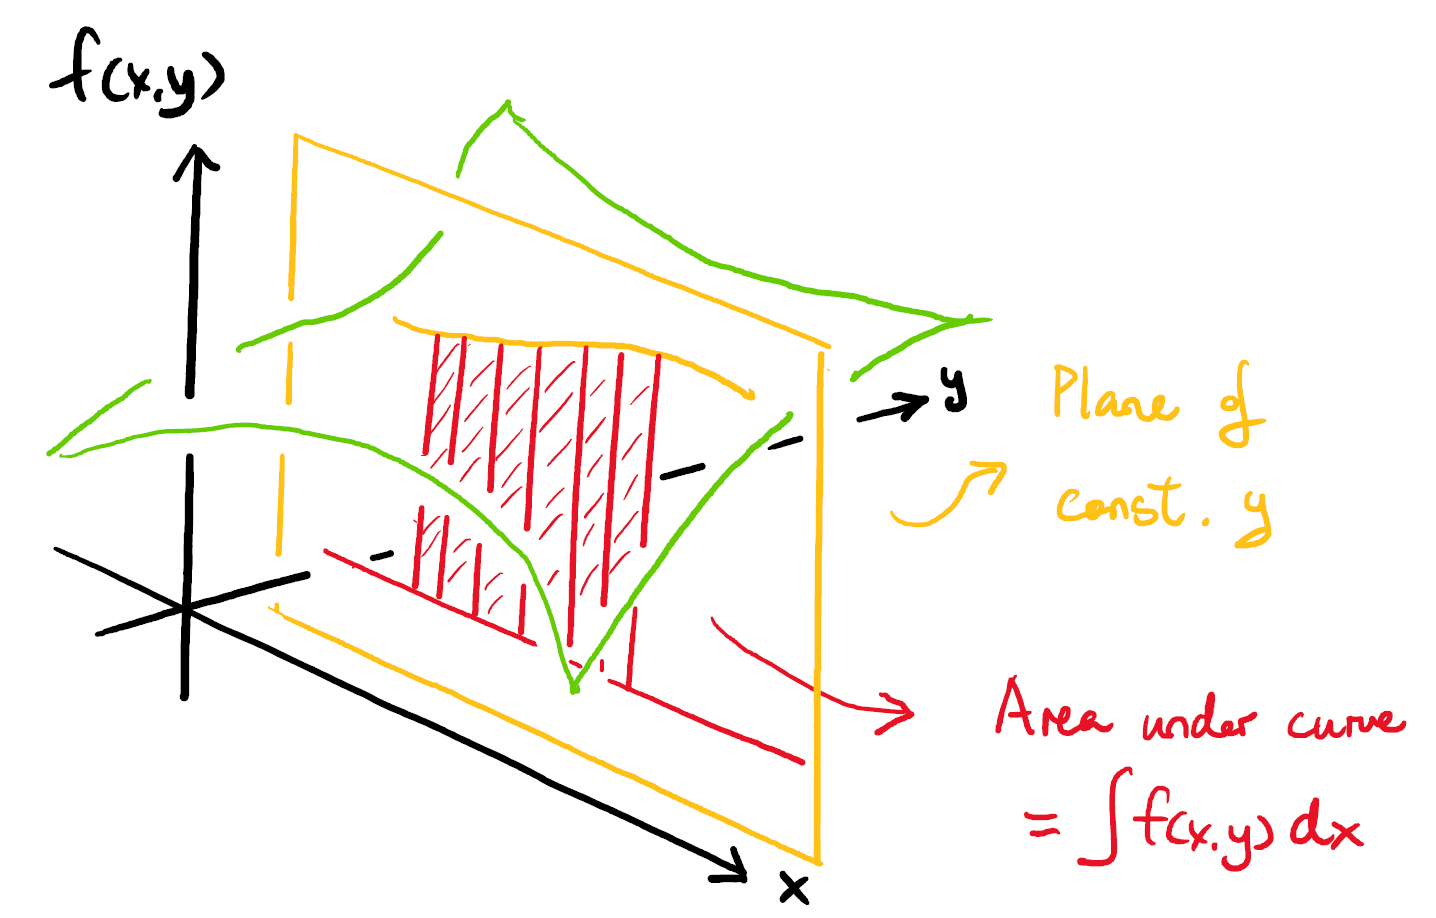
\includegraphics[height=11.5em]{auc_x}
    \end{minipage}
    \hfill\vline\hfill
    \begin{minipage}{0.45\textwidth}
        \centering
       $\displaystyle\int f(x,y)\dd{x} 
        \ =\  \mstack{\text{Integrate along y-axis}\\\text{at constant x}}$\\
        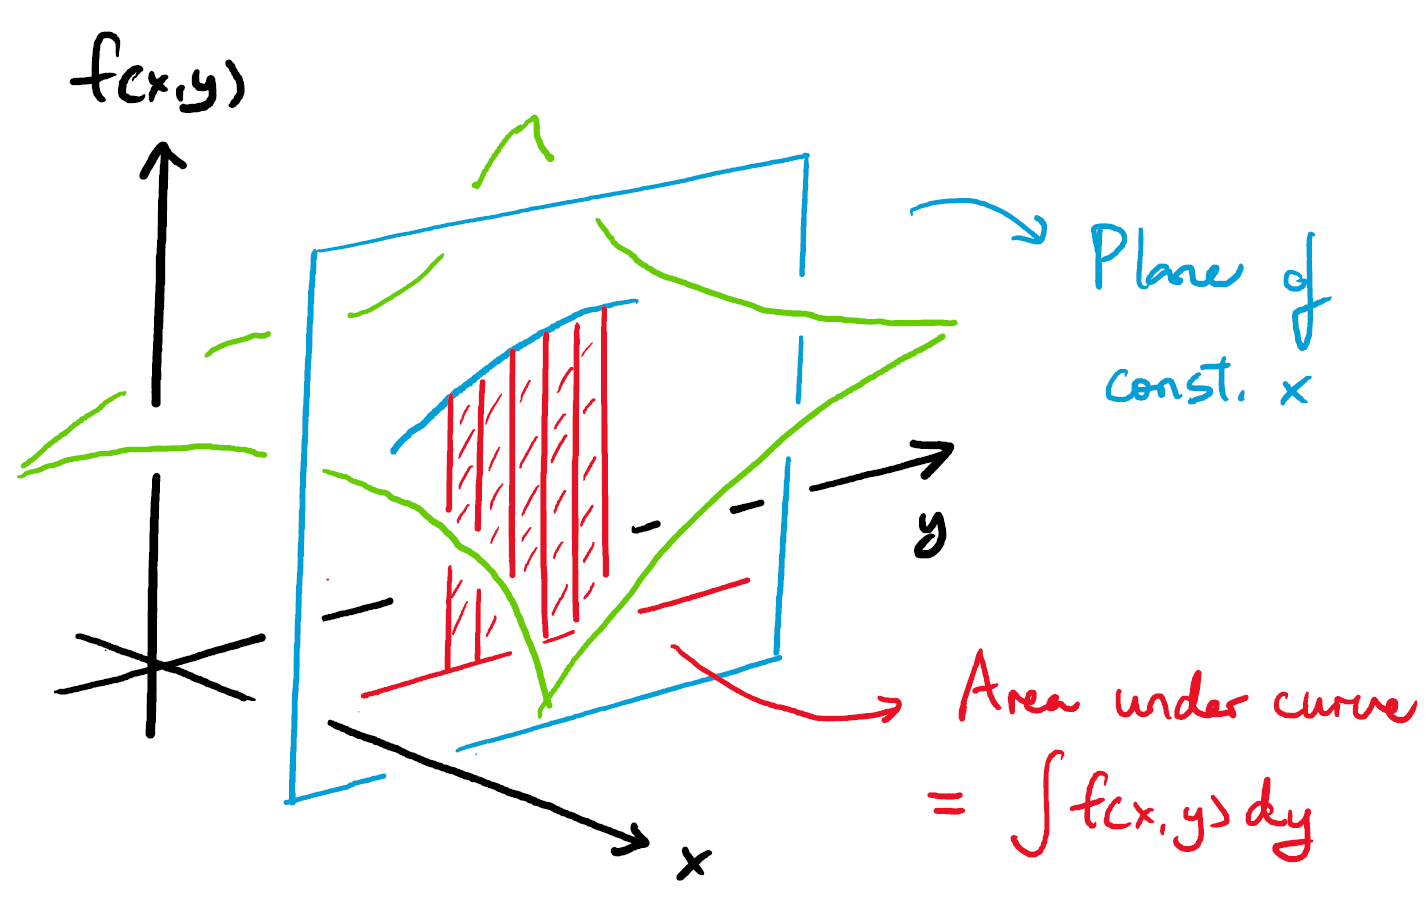
\includegraphics[height=11.5em]{auc_y}
    \end{minipage}
\end{center}

\hfill\\
What about integrating along an arbituary curve?

\begin{center}
    \begin{minipage}{0.6\linewidth}
        \centering
        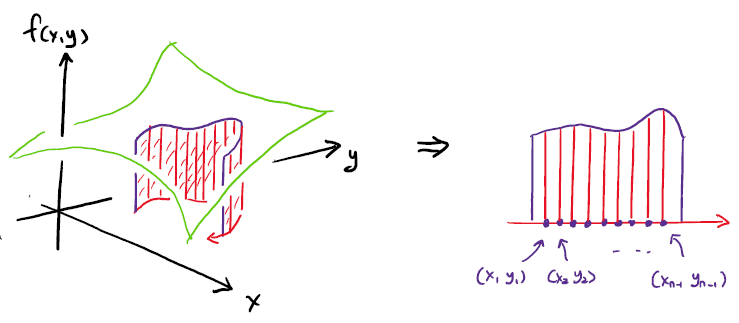
\includegraphics[height=11.5em]{auc_line}
    \end{minipage}
\end{center}

In integration on single variable function, 
we first interpret it as a sum of area under curve.  
We can write something similar for integration along an arbituary curve.\\[1em]
\addBelowArrow[red]{hh}{hhh}{Height of strip}{-3ex}{(0,0)}{(0,-0.5ex)}
\addAboveArrow[blue]{xx}{xxx}{Width of strip}{3ex}
\aleq{
    \int f(x)\dd{x} = \lim_{\Delta x_i\to 0} \sum_{i=1}^n \tkn{hh}{\cul[red]{f(\xi_i)}}\tkn{xx}{\cul[blue]{\Delta x_i}}
    \qquad\Rightarrow\qquad
    \int f(x,y) \dd{\vvec{r}} = \lim_{\norm{\Delta \vvec{r}_i}\to 0} \sum_{i=1}^n \tkn{hhh}{\cul[red]{f(\xi_{i,x}, \xi_{i,y})}}\tkn{xxx}{\cul[blue]{\norm{\Delta \vvec{r}_i}}}
}

\hfill\\[1em]
While the heights of the strips are simply the function's values, 
the widths need to be estimated by Pythegoras theorem.

\begin{center}
    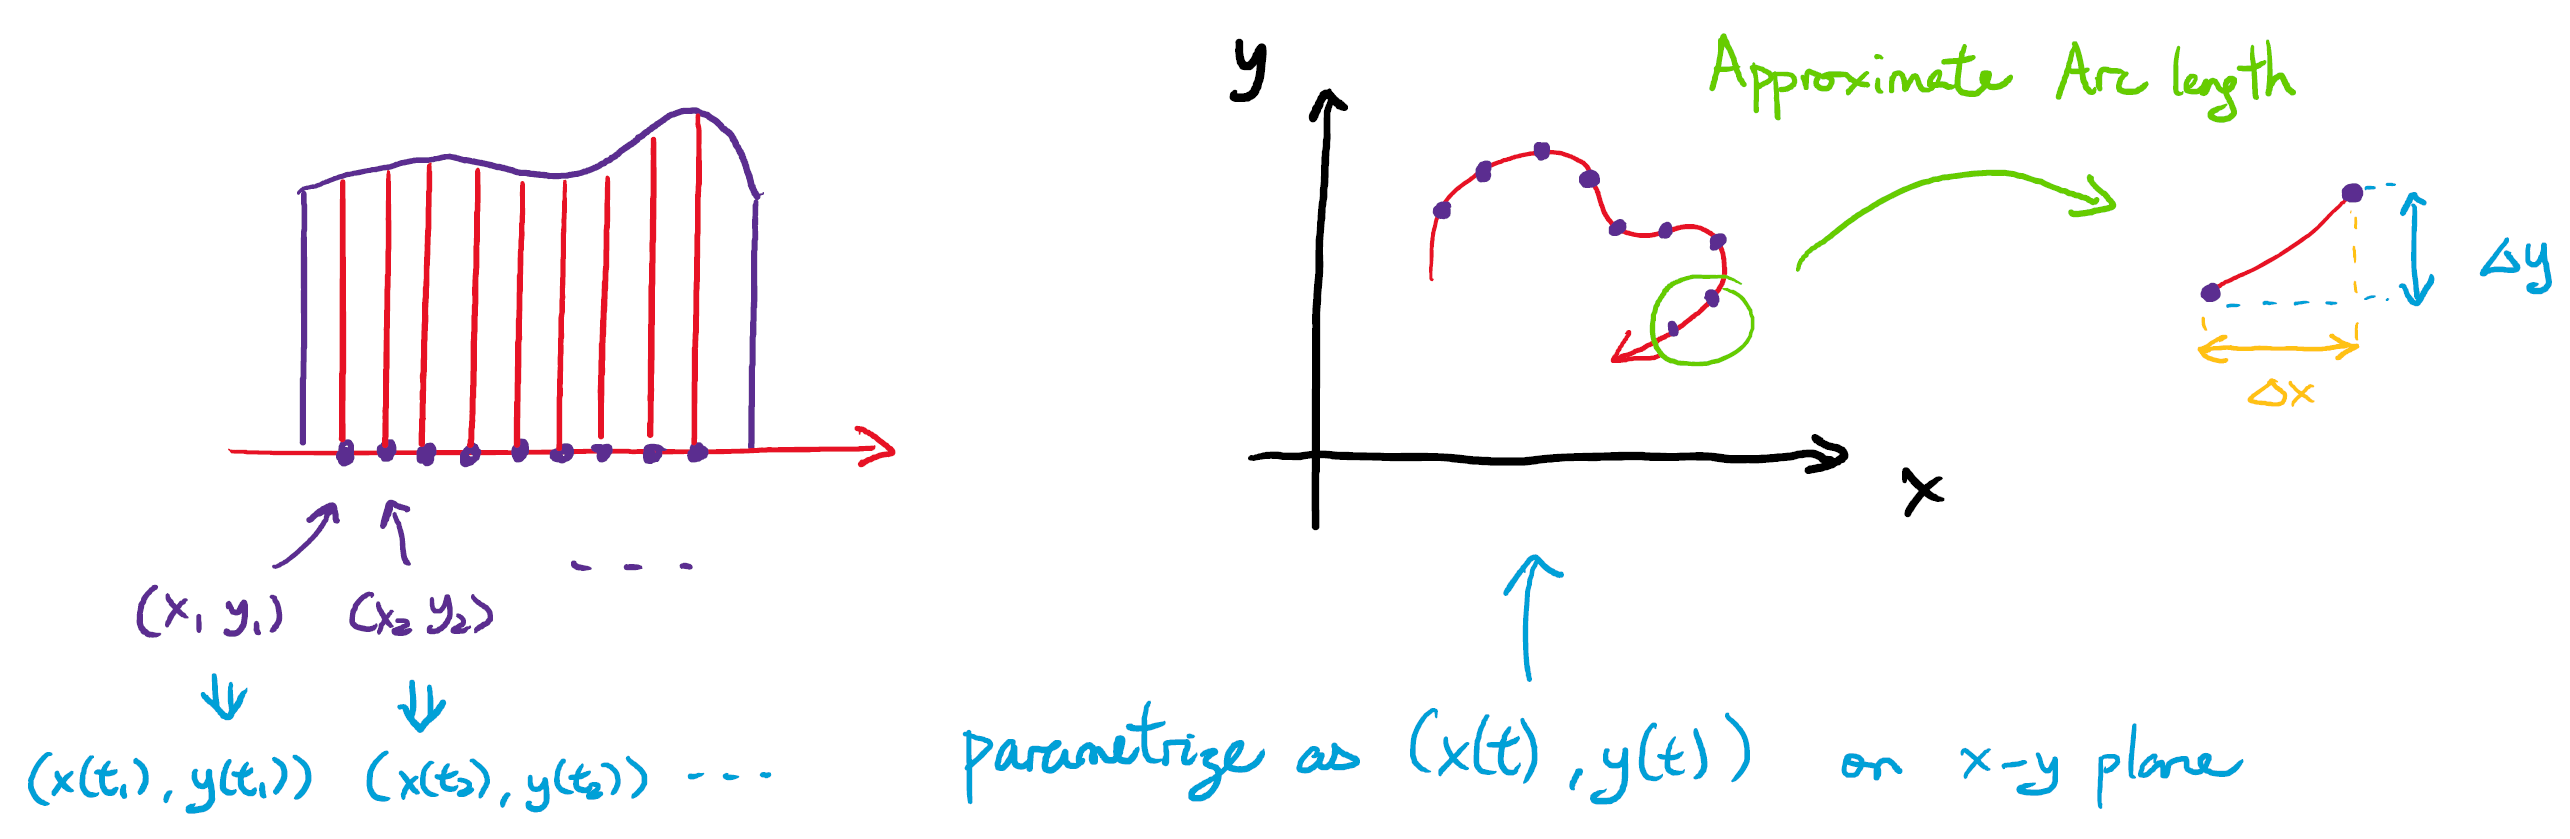
\includegraphics[height=11.5em]{auc_line_para}
\end{center}
\aleq{
    \text{Width of interval }\norm{\Delta \vvec{r}_i}
    &= \sqrt{\qty[x(t_{i+1})-x(t_i)]^2 + \qty[y(t_{i+1})-y(t_i)]^2} \\[1ex]
    &= |t_{i+1}-t_i|\sqrt{\qty[\frac{x(t_{i+1})-x(t_i)}{t_{i+1}-t_i}]^2 + \qty[\frac{y(t_{i+1})-y(t_i)}{t_{i+1}-t_i}]^2} \\[1ex]
    &= |\Delta t_i| \sqrt{\qty[\frac{\Delta x_i}{\Delta t_i}]^2 + \qty[\frac{\Delta y_i}{\Delta t_i}]^2} \\[1ex]
    \lim_{\Delta t_i\to 0}\norm{\Delta \vvec{r}_i} 
    &= \dd{t} \sqrt{\qty(\dvv{x}{t})^2+\qty(\dvv{y}{t})^2}
}

So for the line integral calculation:
\aleq{
    \tkn{text_lineint}{\cbox[blue]{\int f(x,y)\dd{\vvec{r}}}}
    &= \lim_{\norm{\Delta \vvec{r}_i} \to 0} \sum_{i=1}^n f(\xi_{i,x}, \xi_{i,y})\norm{\Delta \vvec{r}_i}\\
    &= \lim_{\Delta t_i \to 0} \sum_{i=1}^n f(\xi_{i,x}, \xi_{i,y})|\Delta t_i| \sqrt{\qty[\frac{\Delta x_i}{\Delta t_i}]^2 + \qty[\frac{\Delta y_i}{\Delta t_i}]^2}\\
    &= \tkn{real_lineint}{\cbox[red]{\int f(x(t),y(t)) \sqrt{\qty(\dvv{x(t)}{t})^2+\qty(\dvv{y(t)}{t})^2}\dd{t}}}
}
\addArrow[blue]{text_lineint}{(0,-3.5ex)}
{\text{The notation}\\\text{you can find}\\in textbook}{(0,-3ex)}{(-2ex,-3ex)}
\addArrow[red]{real_lineint}{(0,-3.5ex)}
{This is how you really calculate line integral\\e.g. along some line on x-y plane.\\(You have to decide how to parametrize the curve!)}
{(0,-3.5ex)}{(0,-3ex)}

\hfill\\[5em]
In addition, We can also interpret line integral as a weighted sum,
like in single variable integral.

\begin{center}
    \begin{minipage}{0.7\linewidth}
        \aleq{
            \int f(\blue{x,y}) \red{\dd{\vvec{r}}} \; 
            \defeq\;  
            \lim_{\Delta x_i \to 0}\, \tkn{s2}{\cul[green]{\sum_{i=0}^{n-1}}}\enspace 
            \tkn{h2}{\cul[blue]{f(\blue{\xi_{i,x}, \xi_{i,y}})}}
            \tkn{w2}{\cul[red]{\red{\norm{\Delta \vvec{r}_i}}}}
        }
    \end{minipage}
    \hspace{0.05\textwidth}
    \begin{minipage}{0.15\linewidth}
        \centering
        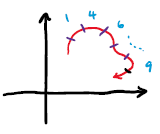
\includegraphics[width=\textwidth]{weight}
    \end{minipage}
\end{center}
\addArrow[green]{s2}{(-5.5ex,-3.5ex)}{\scriptsize Sum\\[-1ex]\scriptsize them all}
{(0,-4ex)}{(-1ex,0)}
\addArrow[blue]{h2}{(0,-4ex)}{\scriptsize "weight"\\[-1ex]\scriptsize assigned to the interval \\[-1ex]\scriptsize $[(x_i, y_i), (x_{i+1},y_{i+1})]$}
{(0,-1.5ex)}{(0,-1.5ex)}
\addArrow[red]{w2}{(8ex,-4ex)}{\scriptsize length of \\[-1ex]\scriptsize interval \\[-1ex]\scriptsize $[(x_i, y_i), (x_{i+1},y_{i+1})]$}
{(0,-1.5ex)}{(2ex,-1.5ex)}

\hfill\\[1em]
\bf{\ul{More on notations}}
\begin{enumerate}
    \item \ul{Extend to N-variables Functions}\\
    The notation for line integral for general multivariable function is by writing the variables in $f$ as a vector $\vvec{r}$
    \aleq{
        \cbox[blue]{\int f(\vvec{r})\dd{\vvec{r}}} \quad\xRightarrow{\text{When calculate}}\quad 
        \cbox[red]{\int f(x_1,...,x_n) \sqrt{\qty(\dvv{x_1}{t})^2+...+\qty(\dvv{x_n}{t})^2}\dd{t}}
    }

    \item \ul{Integration Range}\\
    Single variable integration only requires knowing the upper and lower bounds because the integration range is a straight line.
    However in line integral, we must describe the whole curve, 
    e.g. provide the function of the curve, the starting and ending points, etc.\\
    \aleq{
        \int_a^b f(x)\dd{x} \qquad\Rightarrow\qquad \int_{\substack{\cdots\cdots\cdots\\\text{TL,DR}}}f(\vvec{r})\dd{\vvec{r}}
    }

    This is too many words to write under the integral sign. 
    So conventionally, we just write a symbol $C$ under the integral sign to indicate that this integral is along some curve,
    and then describe the curve in additional texts.
    \aleq{
        \int_C f(\vvec{r})\dd{\vvec{r}} \qquad\text{with}\quad C= \text{Curve of XXX...} 
    }

    \item \ul{Loop Integral}\\
    It is possible that the curve to be integrated along forms a closed loop (e.g. a circle).
    A special symbol is assigned specifically for this use case:
    

    \begin{center}
        \begin{minipage}{0.4\linewidth}
            \aleq{
                \tkn{loop}{\cul[blue]{\oint}} f(\vvec{r})\dd{\vvec{r}}
            }
        \end{minipage}
        \begin{minipage}{0.15\linewidth}
            \centering
            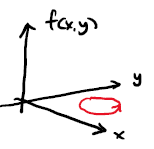
\includegraphics[width=\textwidth]{loop}
        \end{minipage}
    \end{center}
    \addArrow[blue]{loop}{(-5ex,0)}{A circle to represent\\a loop}{(-2ex,0.5ex)}{(-9ex,0)}

    This is because loop integral has some interesting properties and appears in many theorems.
    We shall encounter them later, especially in electrodynamics.

\end{enumerate}

%%%%%%%%%%%%%%
\subsection{Line Integral on Vector Functions}

Observe that $\cul[red]{f(x,y)}\cul[blue]{\dd{r}}$ is a muliplication between a \cul[red]{number} and a \cul[blue]{vector}.
If $f(x,y)$ is to be replaced by a vector function, we have 2 possibilities:
\begin{itemize}
    \item \ul{Dot Product Line Integral}
    \aleq{
        \int \vvec{F}(x,y)\ \cul[green]{\cdot}\ \dd{\vvec{r}} 
        = \lim_{\Delta \vvec{r}_i \to 0} \sum_{i=1}^n \vvec{F}(\xi_{i,x}, \xi_{i,y})\ \cul[green]{\cdot}\ (\Delta \vvec{r}_i)
    }

    \item \ul{Cross Product Line Integral}
    \aleq{
        \int \vvec{F}(x,y)\ \cul[green]{\cross}\ \dd{\vvec{r}} 
        = \lim_{\Delta \vvec{r}_i \to 0} \sum_{i=1}^n \vvec{F}(\xi_{i,x}, \xi_{i,y})\ \cul[green]{\cross}\ (\Delta \vvec{r}_i)
    }
    \red{(Because order matters in cross product, it is quite common to see $\displaystyle \int_C \dd{\vvec{r}}\cross\vvec{F}$)}
\end{itemize}

\hfill\\
\bf{\ul{Calculation}}

Here demonstrates with dot product line integral. 
Cross product is exactly the same.
\addArrow[blue]{dot_int}{(-20ex,-4.5ex)}{}{(0,-2ex)}
\aleq{
    \int \vvec{F}(x,y) \cdot \dd{\vvec{r}} 
    = \lim_{\Delta \vvec{r}_i \to 0} \sum_{i=1}^n \tkn{dot_int}{\cbox[blue]{\vvec{F}(\xi_{i,x}, \xi_{i,y})\cdot (\Delta \vvec{r}_i)}}
}
Notice that this is a summation of \cul[blue]{all dot product} along a curve.
If we express each dot product by the curve parameter $t$: 
\aleq{
    \vvec{F}(x(t_i), y(t_i)) \cdot \Delta\vvec{r}_i 
    &= \vvec{F}(x(t_i),y(t_i))\cdot \qty[\vvec{r}(t_{i+1})-\vvec{r}(t_i)]\\
    &= \vvec{F}(x(t_i),y(t_i))\cdot \qty[\frac{\vvec{r}(t_{i+1})-\vvec{r}(t_i)}{t_{i+1}-t_i}](t_{i+1}-t_i)\\
    &= \vvec{F}(x(t_i),y(t_i))\cdot \qty(\frac{\Delta \vvec{r}_i}{\Delta t_i})\Delta t_i\\
    \lim_{\Delta t_i\to 0} \qty(\vvec{F}(x(t_i),y(t_i))\cdot \Delta\vvec{r}_i) 
    &= \qty(\vvec{F}(x,y)\cdot \dvv{\vvec{r}}{t})\dd{t}
}

So for the line integral calculation:
\aleq{
    \tkn{text_dotint}{\cbox[blue]{\int \vvec{F}(x,y) \cdot \dd{\vvec{r}}}}
    &= \int \vvec{F}(x(t),y(t)) \cdot \qty(\dvv{x(t)}{t}\hhat{x}+\dvv{y(t)}{t}\hhat{y})\dd{t}\\
    &= \tkn{real_dotint}{\cbox[red]{\int \qty[F_x(x(t),y(t))\dvv{x}{t}+F_y(x(t),y(t))\dvv{y}{t}]\dd{t}}}
}
\addArrow[blue]{text_dotint}{(0,-5ex)}
{\text{The notation}\\\text{you can find}\\in textbook}{(0,-3ex)}{(-2ex,-3ex)}
\addArrow[red]{real_dotint}{(0,-5ex)}
{This is how you really calculate line integral\\e.g. along some line on x-y plane.\\(You have to decide how to parametrize the curve!)}
{(0,-4ex)}{(5ex,-3ex)}


\newpage
\bf{\ul{Geometrical intepretation}}\\

The function $\vvec{F}(x,y)$ can be plotted as a "field of vectors",
i.e. at each point $(x,y)$, there is a vector $(F_x,F_y)$

\begin{center}
    \begin{minipage}{0.48\linewidth}
        \centering
        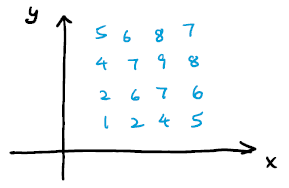
\includegraphics[height=8.5em]{field_scalar}\\
        Scalar function:\\
        Every point is assigned a number\\
    \end{minipage}
    \hfill\vline\hfill
    \begin{minipage}{0.48\linewidth}
        \centering
        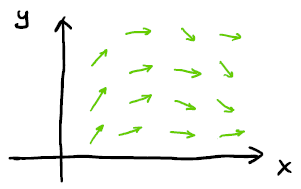
\includegraphics[height=8.5em]{field_vec}\\
        Vector function:\\
        Every point is assigned a vector\\
    \end{minipage}
\end{center}

\hfill\\[1em]
The quantity $\vvec{F}\cdot \dd{\vvec{r}}$ is like,
\begin{itemize}
    \item Find the vector on each segment
    \item Find the interval of each insegment as a displacement vector
\end{itemize}
Then compute the such dot product for each segment and sum them all.

\begin{center}
    \begin{minipage}{0.9\linewidth}
        \centering
        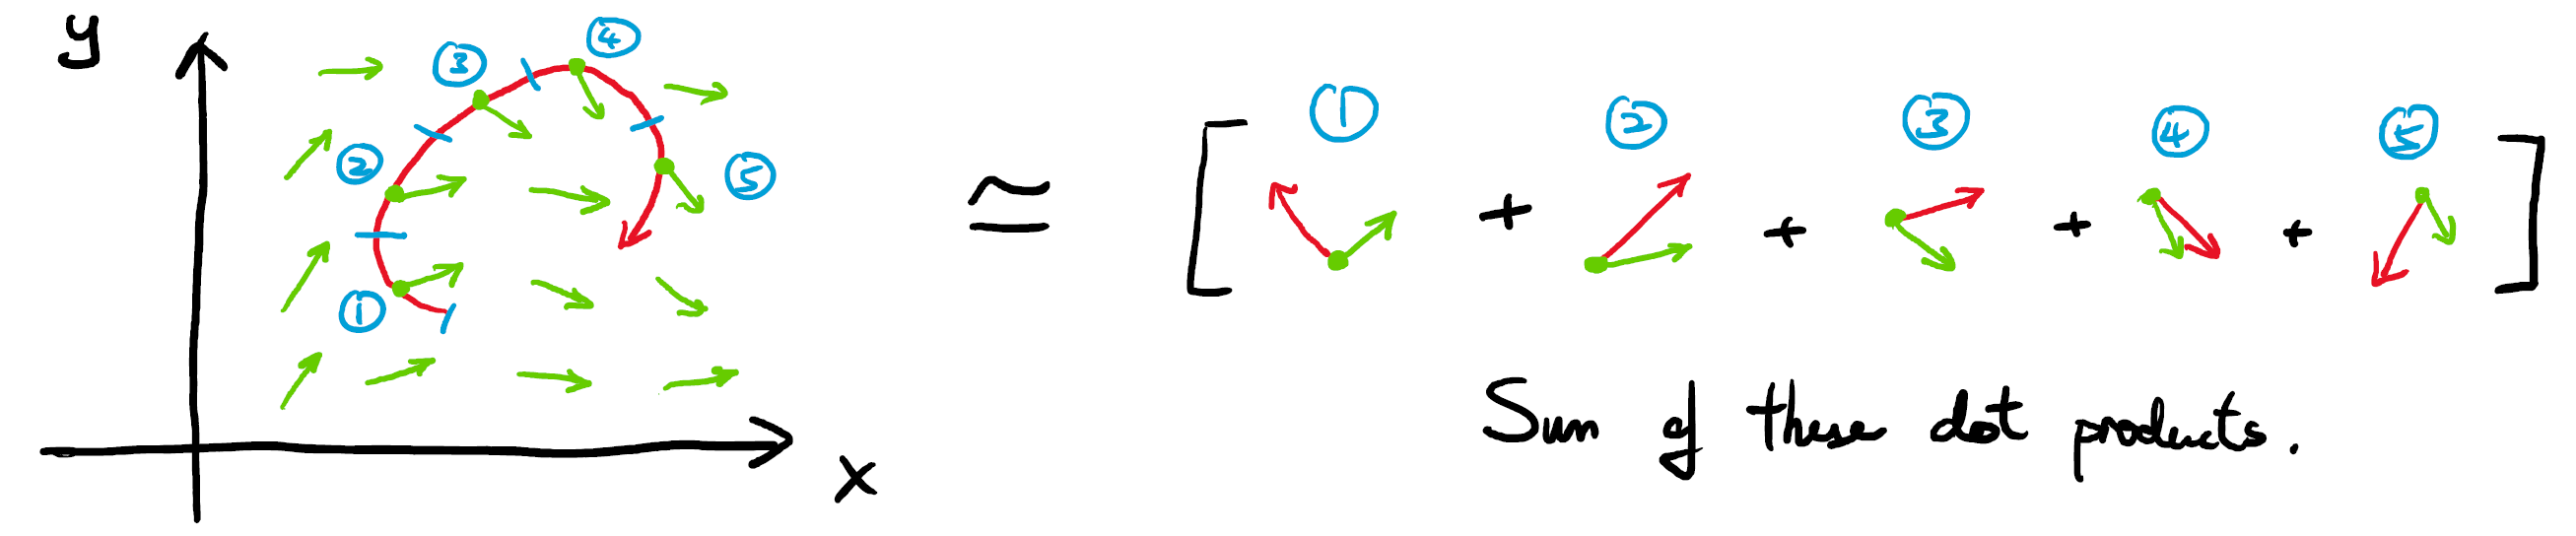
\includegraphics[width=\textwidth]{dot_sum}
    \end{minipage}
\end{center}

\hfill\\
\begin{example}
    An object is moving on a surface with a positional dependent friction force
    \aleq{
        \vvec{F}(x,y) = (x^2y, xy+1)
    }
    Suppose the object is moving in a circular trajectory that is 
    \begin{itemize}
        \item Center at $(1,2)$, radius $=3$
        \item Starts at $(1,5)$, ends at $(4,2)$
        \item Travelling in anticlockwise direction
    \end{itemize}

    Find the W.D. due to friction on this trajectory.

    \newpage
    \begin{enumerate}
        \item Begin with parametrizing the trajectory
        \begin{center}
            \begin{minipage}{0.65\linewidth}
                \centering
                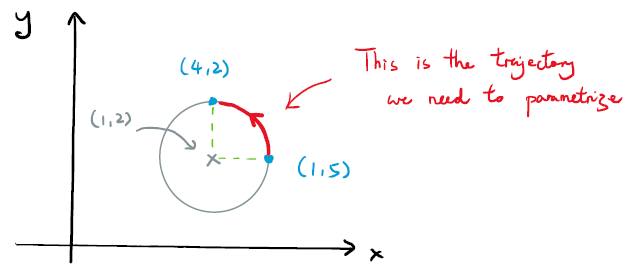
\includegraphics[width=\textwidth]{curve_para_eg}
            \end{minipage}
        \end{center}


        Recall that parametrization for circle is usaully in the from
        \aleq{
            \bcase{
                x(\theta) &= x_0 + R\cos(\theta+\phi)\\
                y(\theta) &= y_0 + R\sin(\theta+\phi)
            }
        }

        From the given information, we can identify
        \aleq{
            (x_0,y_0)&=(2,1) \quad,\quad R=3 \quad,\quad \phi=0\\
            &\Rightarrow
            \bcase{
                x(\theta) &= 2+3\cos\theta\\
                y(\theta) &= 1+3\sin\theta
            }
        }
        The start/end correspond to 
        \aleq{
            \bcase{
                \theta=0 \quad\Leftrightarrow\quad (x,y)=(5,1)\\
                \theta=\frac{\pi}{2} \quad\Leftrightarrow\quad (x,y)=(2,4)
            }
        }

        \item Substitute into the dot product line integral
        \aleq{
            \text{W.D.} &= \int_C \vvec{F}\cdot \dd{\vvec{r}}\\
            &= \int_C \vvec{F}(x,y) \cdot \dvv{\vvec{r}(\theta)}{\theta} \dd{\theta} \\
            &= \int_{\red{\theta=0}}^{\red{\theta=\frac{\pi}{2}}} \bmat{x^2y & xy+1}
                \dvv{\theta}\bmat{x \\ y} \dd{\theta}\\
            &= \int_{\red{\theta=0}}^{\red{\theta=\frac{\pi}{2}}} \qty[x^2y\dvv{x}{\theta} + (xy+1)\dvv{y}{\theta}]\dd{\theta}\\
            &= \int_{\red{\theta=0}}^{\red{\theta=\frac{\pi}{2}}} \qty[\cut[blue]{(1+3\cos\theta)^2}{x^2}\cut[blue]{(2+3\sin\theta)}{y}\cut[blue]{(-3\sin\theta)}{\dv{x}{\theta}}
                + \qty[\cut[blue]{(1+3\cos\theta)}{x}\cut[blue]{(2+3\sin\theta)}{y}\cut[blue]{+1}{+1}]\cut[blue]{3\cos\theta}{\dv{y}{\theta}}] \dd{\theta}\\
            &= \cdots
        }
        
        The remaining steps are just solving an annoying single variable integration, 
        which you all should know how to do so.
    \end{enumerate}
\end{example}

%%%%%%%%%%%%%%
\subsection{Gradient Theorem}

If $f(\vvec{r})$ is a \ul{continuous scalar function}, 
and $\grad f(\vvec{r})$ is its gradient vector (field), 
then the line integral

\hfill\\[-3.5em]
\begin{center}
    \begin{minipage}{0.55\linewidth}
        \aleq{
            \int_{\red{\substack{\text{start}\\\text{from }\vvec{r}_1}}}^{\red{\substack{\text{end}\\\text{at }\vvec{r}_2}}}
                \grad f(\vvec{r}) \cdot \dd{\vvec{r}} 
            = f(\red{\vvec{r}_2}) - f(\red{\vvec{r}_1})
        }
    \end{minipage}
    \begin{minipage}{0.4\linewidth}
        \centering
        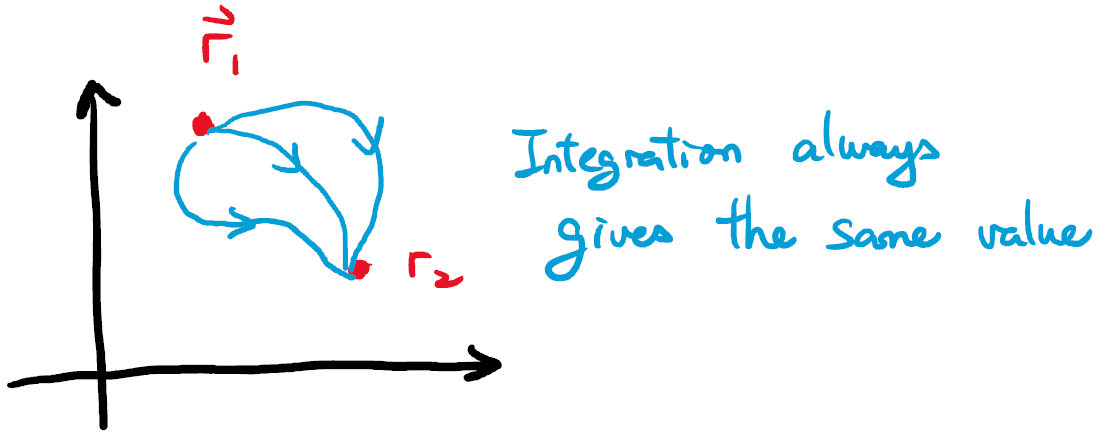
\includegraphics[width=\textwidth]{int_path}
    \end{minipage}
\end{center}

is \ul{independent of what curve we are integrating along}.

\begin{center}
    (We can skip all the steps of curve parametrization!)\\
\end{center}


To illustrate, recall that $\grad f\cdot \hhat{u} =$ slope in $\hhat{u}$'s direction.
So,


\begin{center}
    \begin{minipage}{0.6\linewidth}
        \aleq{
            \grad f \cdot \dd{\vvec{r}} 
            &= \grad f \cdot \cut[blue]{\cbox[blue]{\frac{\dd{\vvec{r}}}{\norm{\dd{\vvec{r}}}}}}{\text{unit vector}}\norm{\dd{\vvec{r}}}\\[1ex]
            &= \qty(\mstack{\text{slope in}\\\dd{\vvec{r}}\text{ direction}})\times \qty(\mstack{\displaystyle\text{Base}\\\displaystyle\text{length}})\\[1em]
            &= \qty(\mstack{\text{Change in height} \\ \text{along }\dd{\vvec{r}}})
        }
    \end{minipage}
    \begin{minipage}{0.38\linewidth}
        \centering
        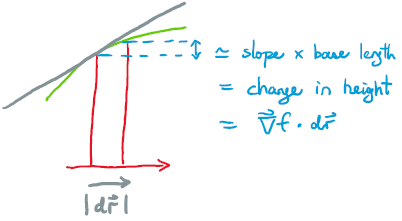
\includegraphics[width=\textwidth]{int_slope}
    \end{minipage}
\end{center}

Therefore,
\aleq{
    \int_{\substack{\text{start}\\\text{from }\vvec{r}_1}}^{\substack{\text{end}\\\text{at }\vvec{r}_2}}
        \grad f(\vvec{r}) \cdot \dd{\vvec{r}}
    &= \text{Sum of all }\grad f\cdot\dd{\vvec{r}} \text{ along a curve from } 
        \vvec{r}_1 \text{ to } \vvec{r}_2 \\
    &= \text{Net height change by travelling from }\vvec{r}_1 \text{ to }\vvec{r}_2
}

And this should be intuitive - when the landscape is continuous,
the net height change should be always independent of which path is taken.

\begin{center}
    \begin{minipage}{0.35\linewidth}
        \centering
        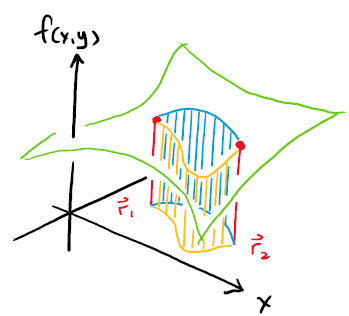
\includegraphics[width=\textwidth]{int_height}
    \end{minipage}
\end{center}


%%%%%%%%%%%%%%
\subsection{Application: Conservative Force \& Potential}

Any vector function $\vvec{F}(\vvec{r})$ is \bf{conservative} 
if it equals to the gradient vector of some scalar function $U(\vvec{r})$.
\aleq{
    \tkn{force}{\vvec{F}(\vvec{r})} = \tkn{minus}{-}\grad \tkn{PE}{U(\vvec{r})}
}
\addArrow[red]{force}{(-8ex,-4ex)}{Vector field\\= the force}{(-1ex,-1ex)}{(-5ex,-1ex)}
\addArrow[green]{minus}{(0,-4ex)}{Have a minus sign\\by definition}{(0,-1ex)}{(0,-2ex)}
\addArrow[blue]{PE}{(12ex,-4ex)}{Scalar function\\= the potential energy}{(0,-1ex)}{(5ex,-1ex)}

\hfill\\[2em]
If the force's vector field is conservative, it has a nice property:
\aleq{
    \mstack{\text{Total W.D. along}\\\text{any path between }\vvec{r}_1,\vvec{r}_2}
    &= \int_{\vvec{r}_1\to\vvec{r}_2} \vvec{F}\cdot\dd{\vvec{r}}\\[1em]
    &= \int_{\vvec{r}_1\to\vvec{r}_2} -\grad U\cdot \dd{\vvec{r}}\\[1em]
    &= - (U(\vvec{r}_2) - U(\vvec{r}_1))
}

Because of gradient theorem, all we need to know are just the start and end points.
Taking any path will cost the same work done.

\begin{example}
    We all know that gravitional force is a conservative vector function. 
    \aleq{
        \vvec{F}(\vvec{r}) = \frac{GMm}{\norm{\vvec{r}}^2} 
    }

    \hfill\\[-3.5em]
    \begin{center}
        \begin{minipage}{0.8\linewidth}
            which is why we can compute the gravitational potential energy change by
            \aleq{
                \Delta U(\vvec{r}) = -\int_{\vvec{r}_1\to\vvec{r}_2} \vvec{F}\cdot\dd{\vvec{r}}
                = -\qty(\frac{GMm}{\norm{\vvec{r}_2}} - \frac{GMm}{\norm{\vvec{r}_2}} )
            }
        \end{minipage}
        \begin{minipage}{0.15\linewidth}
            \centering
            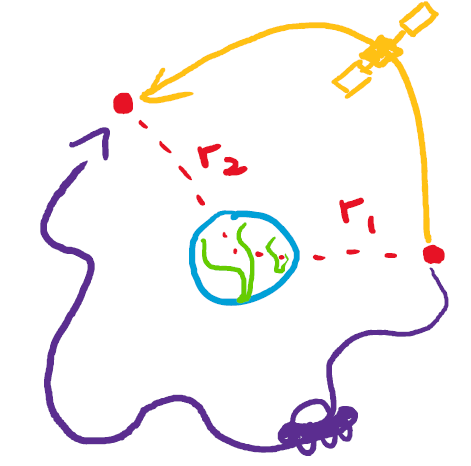
\includegraphics[width=\textwidth]{ufo}
        \end{minipage}
    \end{center}
    
    without EVER doing annoying line integral. 
    (And so it can appear in your high school syllabus)


\end{example}

\begin{notation}[Side note:]
    To prove that a force field is conservative, 
    we have to show that its \it{curl = 0}, i.e.
    \aleq{
        \curl \vvec{F} = 0
    }
    However we will not touch this devil until E\&M.
\end{notation}


%%%
\theend
\end{document}